\section{4W联合统计结果}\label{sec:4w_combination}

为了最大化4W分析道的灵敏度,
对3个现有衰变分析道进行统计组合,包括2LSS,3Lep和4Lep。
统计处理与参考文献~\cite{Aad:2012an,ATLAS:2011tau}中描述的相同。
每个bin的事例数采用泊松假设,联合乘积即可构建似然函数;
其中系统误差,即冗余参数,利用高斯函数模拟。
值得注意的是,影响多个分析道的系统误差应当使用相同的冗余参数,这样子系统误差对整个实验
的影响才能有效一致的传递。
检验统计量使用参考文献~\cite{Cowan:2010js}中定义的profile似然比$\Lambda(\mu)$。
最终应用渐近逼近式修改的频率方法在95\% CL$_s$~\cite{CLs_2002}置信度下提取上限。

\subsection{系统误差关联性}
影响多个衰变分析道的系统误差关联考虑,具体关联情况见表~\ref{comb:SysCorr}。
\begin{table}
\centering
\scriptsize\scalebox{0.8}{
\begin{tabular}{c|c|c}
\hline
   Sys source   &number of NP   &correlation strategy\\
\hline
   Lumi         & 1NP           & {\color{blue}{correlated}}\\
\hline
   Jet systematic & JES 21NP \footnote{JES is not correlated according to \href{https://twiki.cern.ch/twiki/bin/view/AtlasProtected/JetUncertainties20152016Data20p7\#Globally_reduced\_21\_parameter\_20}{\color{blue}{this link}}}, JER 1NP &{\color{red}{21NP JES is not correlated}}, {\color{blue}{JER is correlated}}\\
\hline
   EGam systematic & EG Scale 1NP, EG resolution 1NP &{\color{blue}{correlated}}\\
\hline
   Electron systematic & 4(ID,RECO,TRIG,ISO) for SS2L/3L, 33(15 uncorr+15corr+3 ISO, reco, TRIG) for 4L &{\color{blue}{only correlate SS2L and 3L}}\\
\hline
   Muon systematic & Trigger(2NP),ID(4),TTVA(2NP),ISO(2NP),Momentum(3NP) & {\color{blue}{correlated}}\\
\hline
   Flavor tagging & 6(B)+4(C)+15(Light)+2(Extrap) & {\color{blue}{correlated}}\\
\hline
   MET  & 3NP     & {\color{blue}{correlated}} \\
\hline
   Pileup &1NP & {\color{blue}{correlated}}\\
\hline
   MC Stat &    & {\color{red}{not correlated}}\\
\hline
   Fake factor uncertainty&6(2L)+2(3L)+1(4L)     & {\color{red}{not correlated}}\\
\hline
\end{tabular}}
\caption{4W分析中各种系统误差关联策略。}
\label{comb:SysCorr}
\end{table}
亮度,$\mu$ 子,轻子,光子,味道鉴别,pile-up和MET相关的系统误差是相互关联的,而fakes相关的误差没有关联,因为fakes是在不同的区域估计的。
%JES uncertainty is not correlated because the knowledge of the source is removed when the simplification of nuisance parameter scheme is done?
%The uncertainty on the electron efficiency is only correlated between 2L and 3L channels, since 4L uses a different correlation scheme.?

\subsection{统计模型检查}
本节检查建立的统计模型中的NP在数据影响下的偏移(pull),NP相关性以及影响排序。为了使得图像更清晰,所有的pull图分为两张,其中红点是4Lep中的$ZZ$归一因子,因为它并不是高斯函数所模拟,所以其中心值为1,在联合拟合中的误差大约为5\%。

图~\ref{fig:pull-exp-comb-260}到图~\ref{fig:pull-exp-comb-500_mu1}展示在$m_X$=260 GeV和$m_X$=500 GeV两个质量点搜寻中系统误差在不同假设下的拟合结果。在无信号假设和S+B的假设下,pull的表现是非常合理的。
而在实际观测数据的拟合中,因为数据的涨落,2L的fakes误差偏移较大。在图~\ref{fig:corr-comb-260}和图~\ref{fig:corr-comb-500}还可以看到,系统误差之间没有较大相关性。
图~\ref{fig:rank-comb-260}和图~\ref{fig:rank-comb-500}是系统误差影响的排序,虚线阴影区表示截面上限随NP向上或向下变化一个标准偏差时的变化,并分别展示拟合前和拟合后的变化情况。
fake factor的系统误差对最终结果影响最大。在$m_X$=500 GeV的S+B asimov拟合和观测值拟合中,\texttt{JET Pileup OffsetMu}对3L只有单边的影响,这是源于其对信号和本底
的影响是单边的,见表\ref{tab:Variation_Pileup_OffsetMu}。
\begin{table}
\scriptsize\scalebox{0.7}{
\centering
\begin{tabular}{c|c|c|c|c|c}
\hline
alpha\_ATLAS\_JET\_21NP\_JET\_Pileup\_OffsetMu  &\multicolumn{2}{c}{background}    &\multicolumn{2}{c}{signal}&observed \\
\hline
ThreeLep\_SFOS0\_m500   &0.000(+1$\sigma$)/-0.004(-1$\sigma$)(in percentage)     &0.00/-0.00(yield)      &-0.490(+1$\sigma$)/-0.001(-1$\sigma$)   &-0.18/-0.00(yield)&2\\
\hline
ThreeLep\_SFOS12\_m500  &0.000(+1$\sigma$)/0.000(-1$\sigma$)(in percentage)      &0.00/0.00(yield)       &-0.485(+1$\sigma$)/0.006(-1$\sigma$)    &-0.43/0.01(yield)&1\\
\hline
\end{tabular}}
\caption{系统误差\texttt{JET\_Pileup\_OffsetMu}对信号本底的相对影响,其正反变化不对称。}
%\caption{Systematic variation on signal and total background yield. The variation is asymmetric on signal yield.}
\label{tab:Variation_Pileup_OffsetMu}
\end{table}

\begin{figure}
\centering
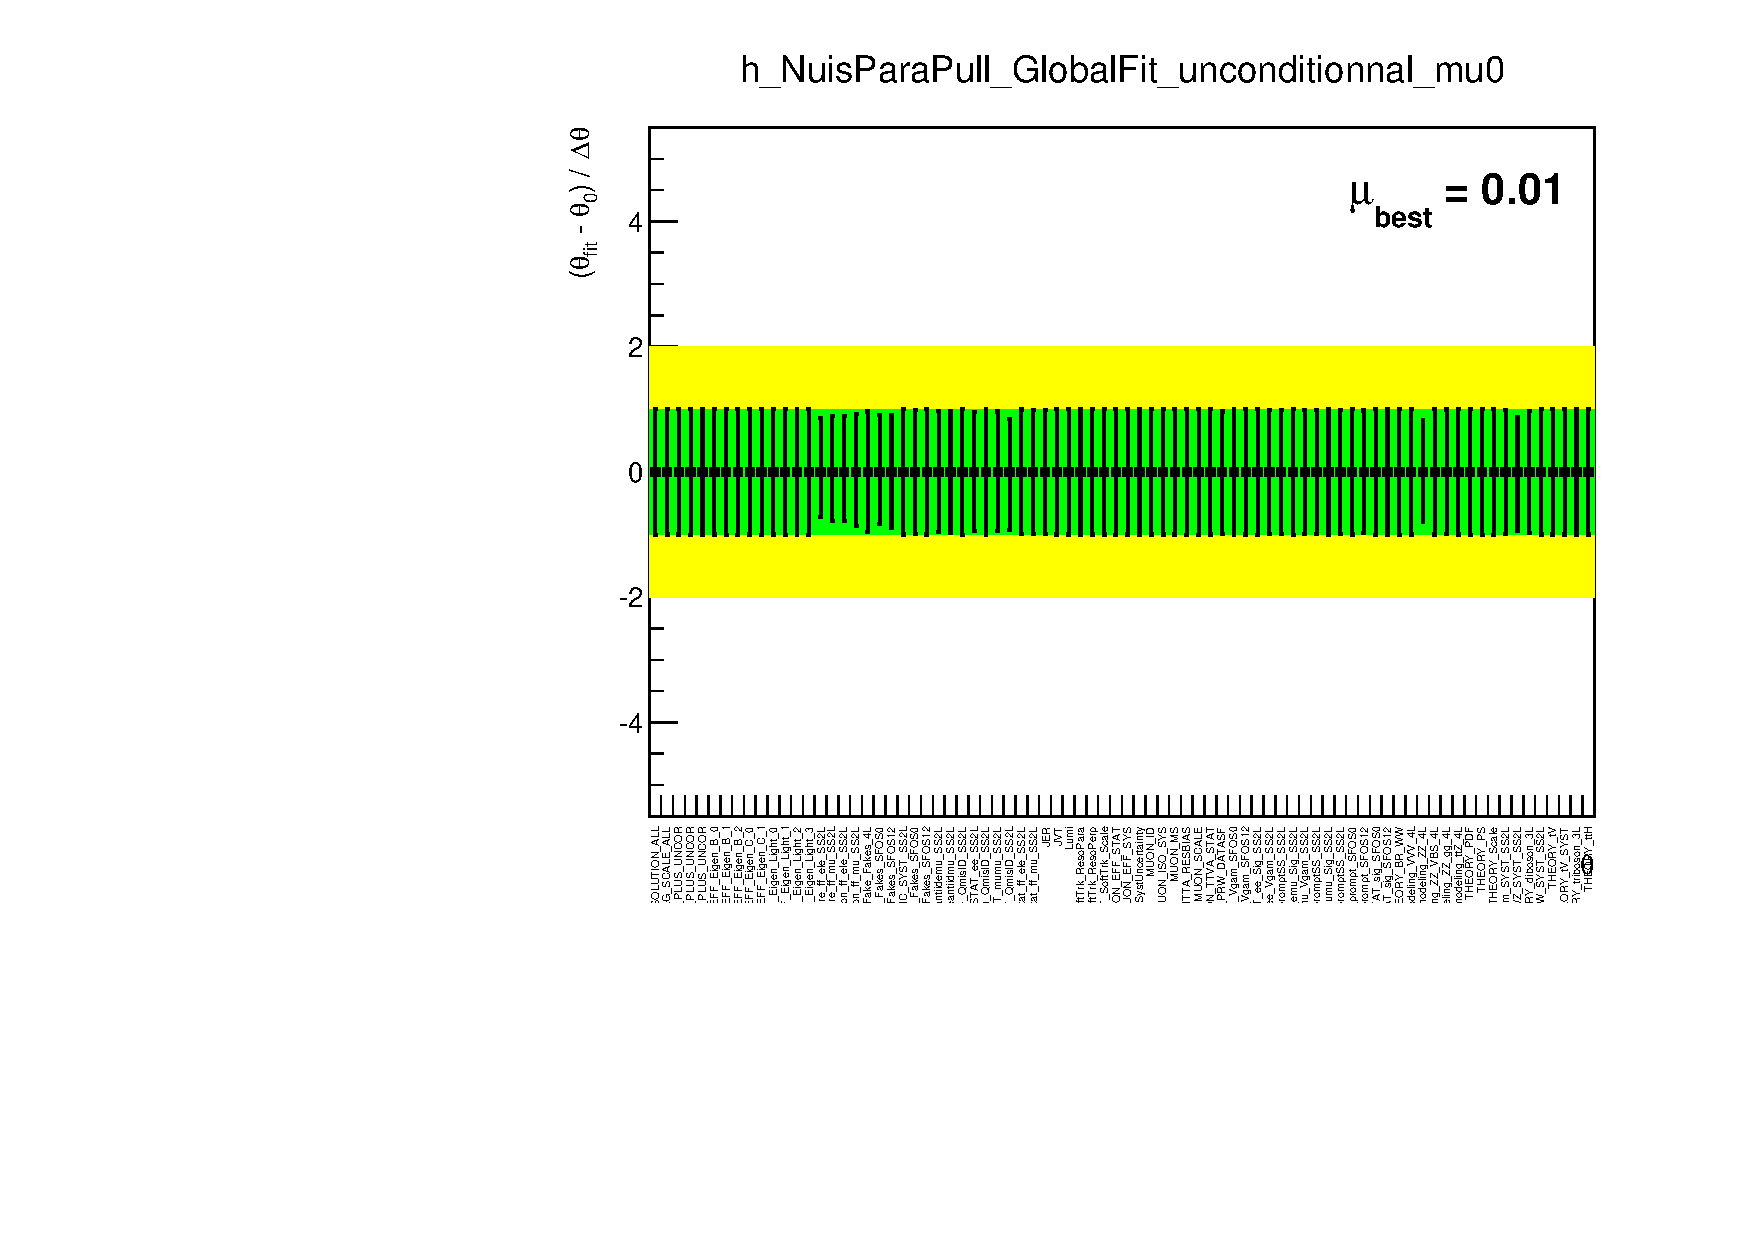
\includegraphics[width=.35\textwidth, angle=-90]{fig/Statistical/combination/pull-exp-combined-mH260_1.pdf}
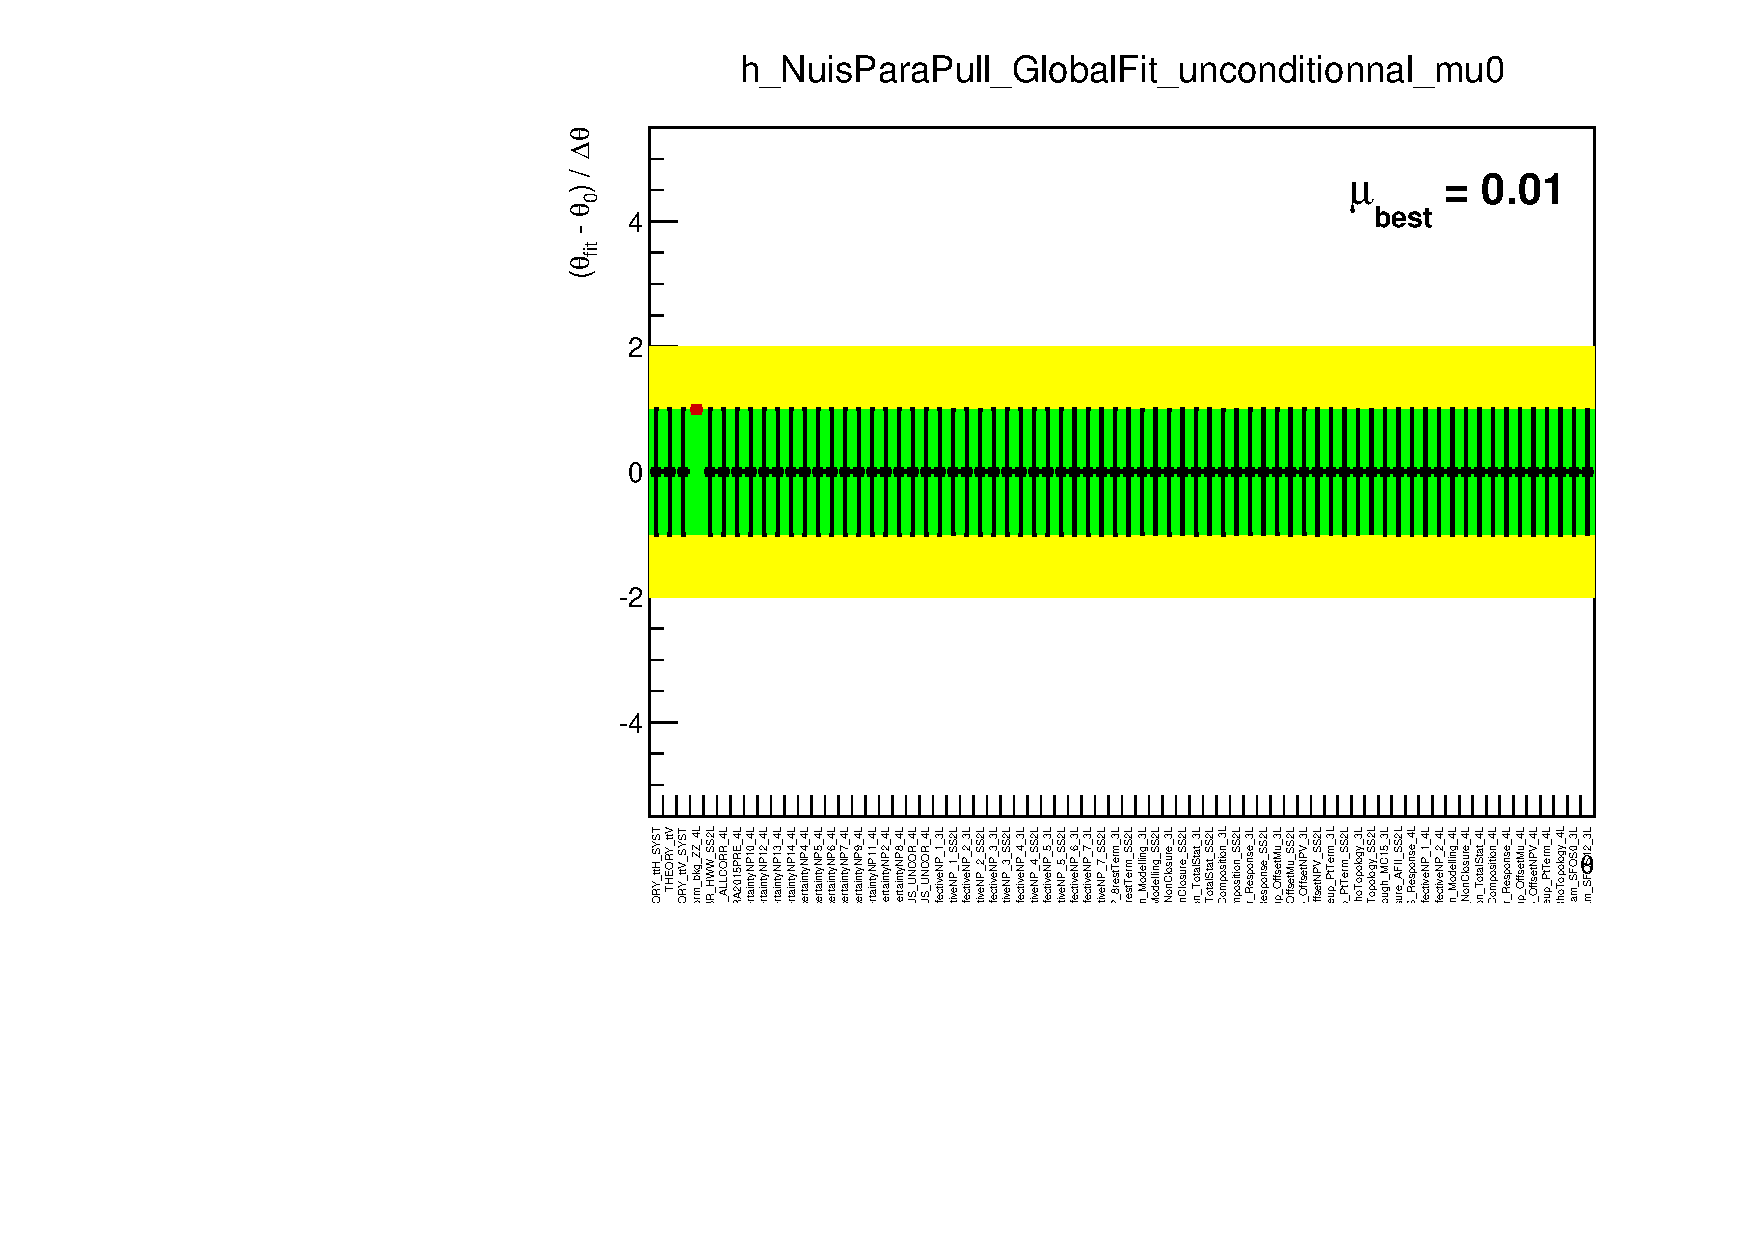
\includegraphics[width=.35\textwidth, angle=-90]{fig/Statistical/combination/pull-exp-combined-mH260_2.pdf}
%\caption{pull check on B-only asimovData of $m_{H}=260 GeV$}
\caption{无信号Asimov数据给出的$m_X$=260 GeV pull图。}
\label{fig:pull-exp-comb-260}
\end{figure}


\begin{figure}
\centering
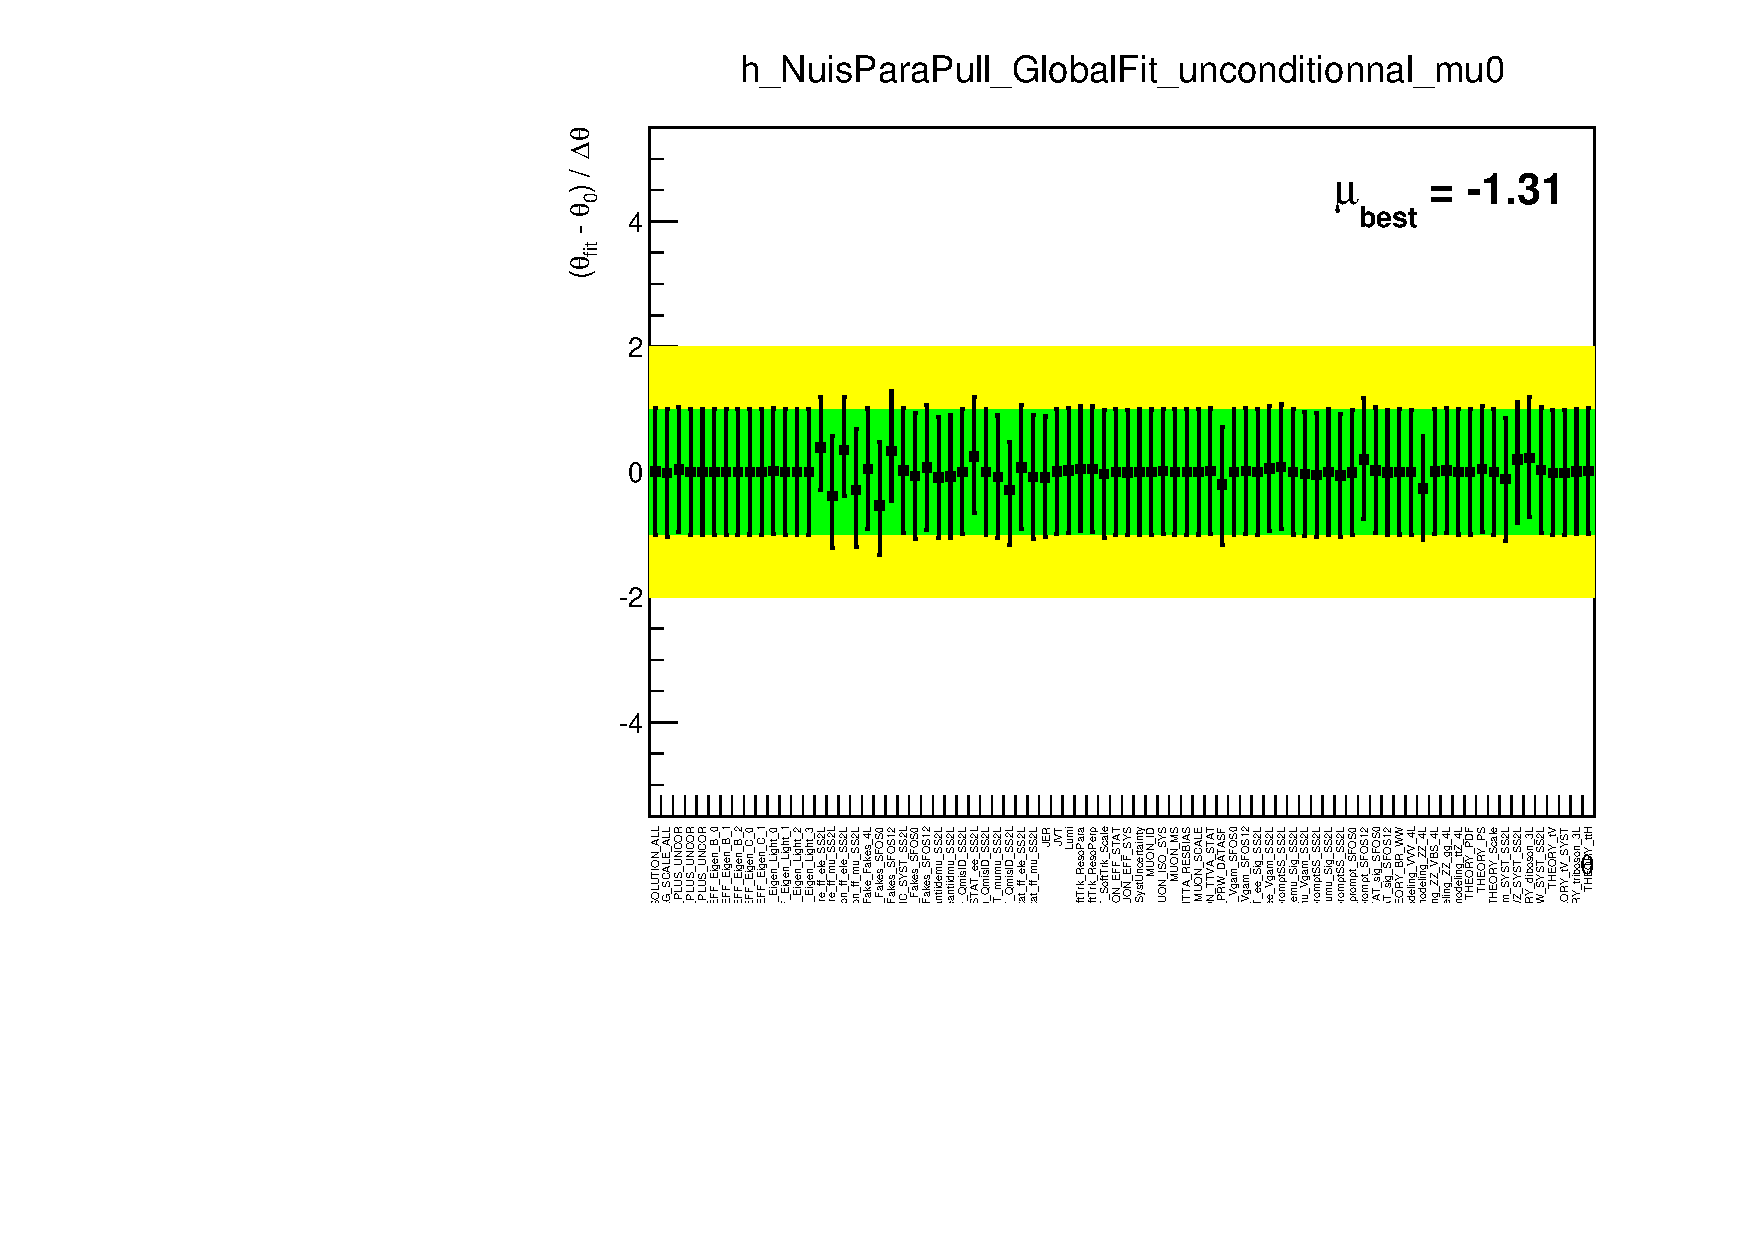
\includegraphics[width=.35\textwidth, angle=-90]{fig/Statistical/combination/pull-obs-combined-mH260_1.pdf}
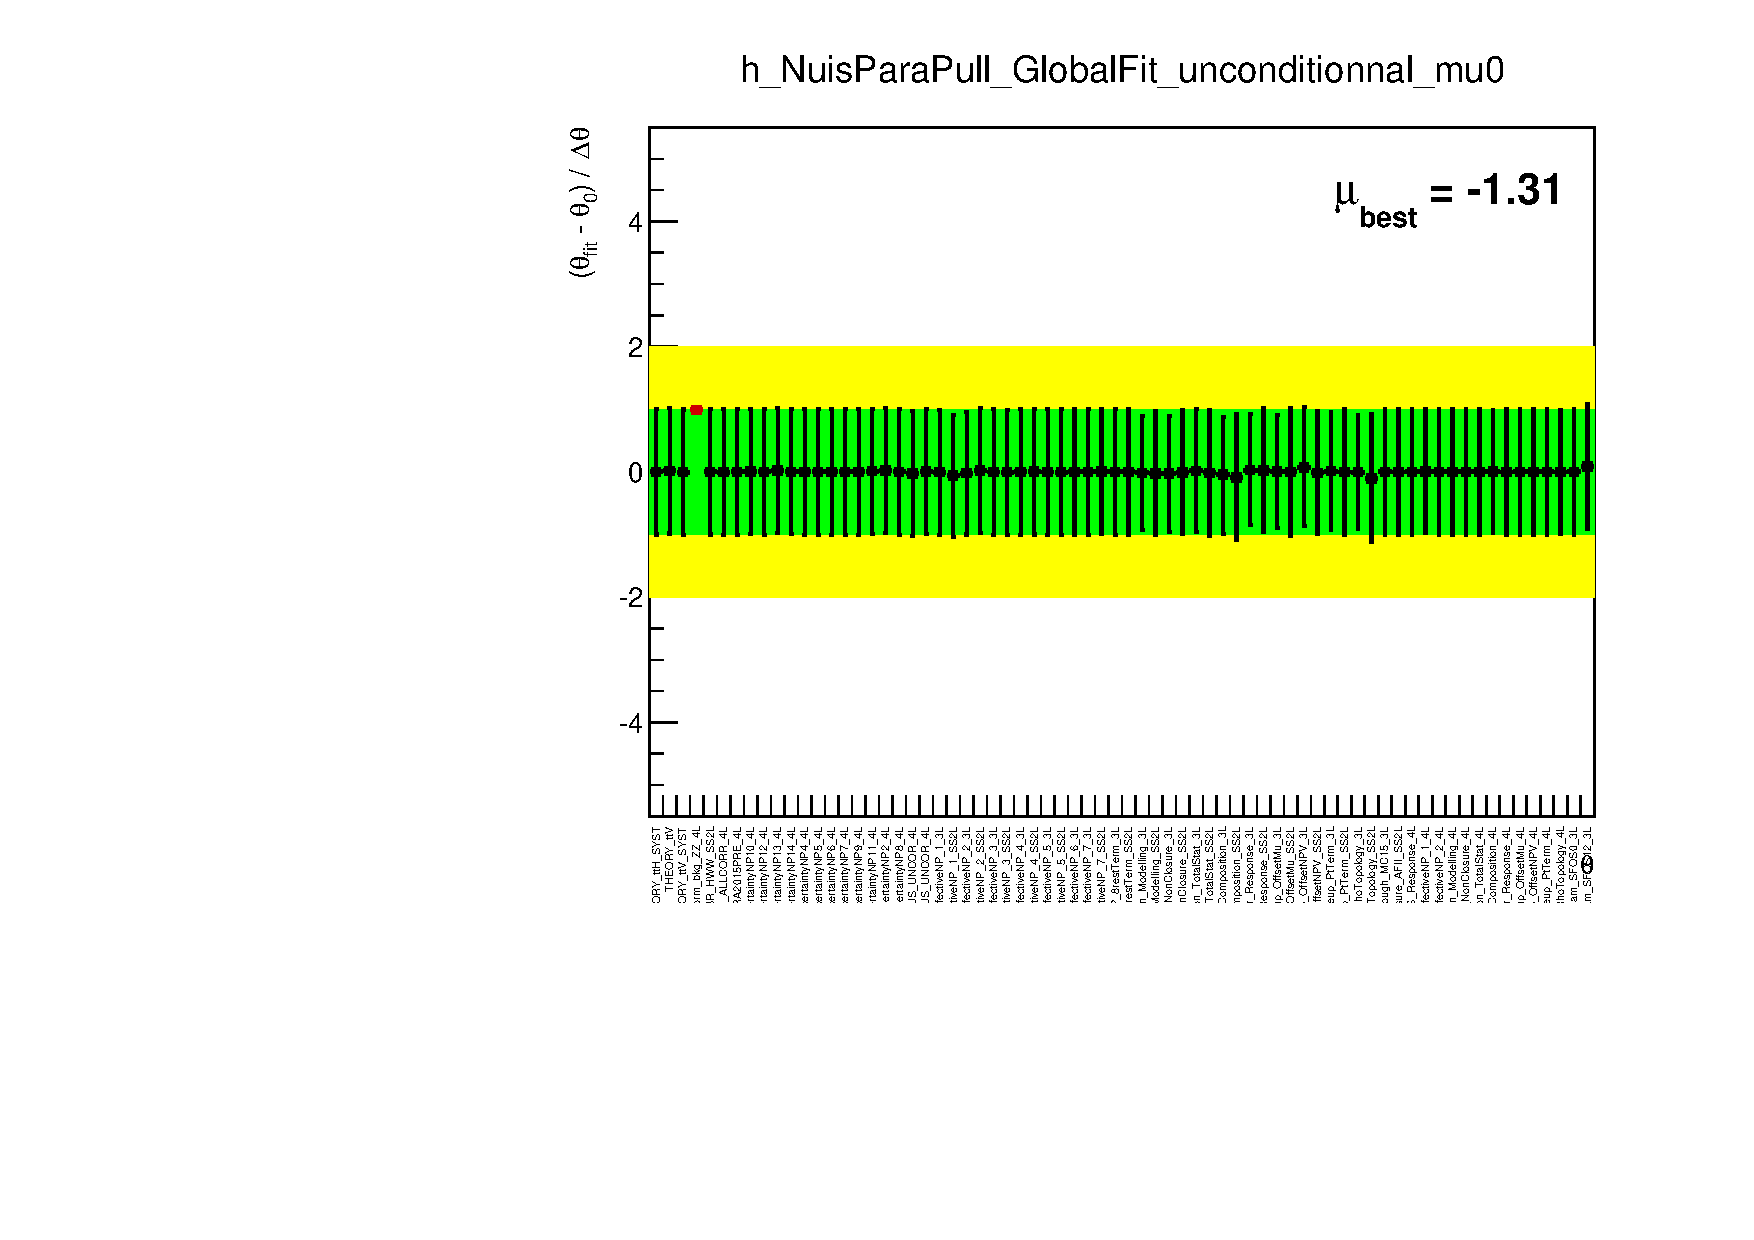
\includegraphics[width=.35\textwidth, angle=-90]{fig/Statistical/combination/pull-obs-combined-mH260_2.pdf}
%\caption{pull check on obsData of $m_{H}=260 GeV$}
\caption{观测数据给出的$m_X$=260 GeV pull图。}
\label{fig:pull-obs-comb-260}
\end{figure}

\begin{figure}
\centering
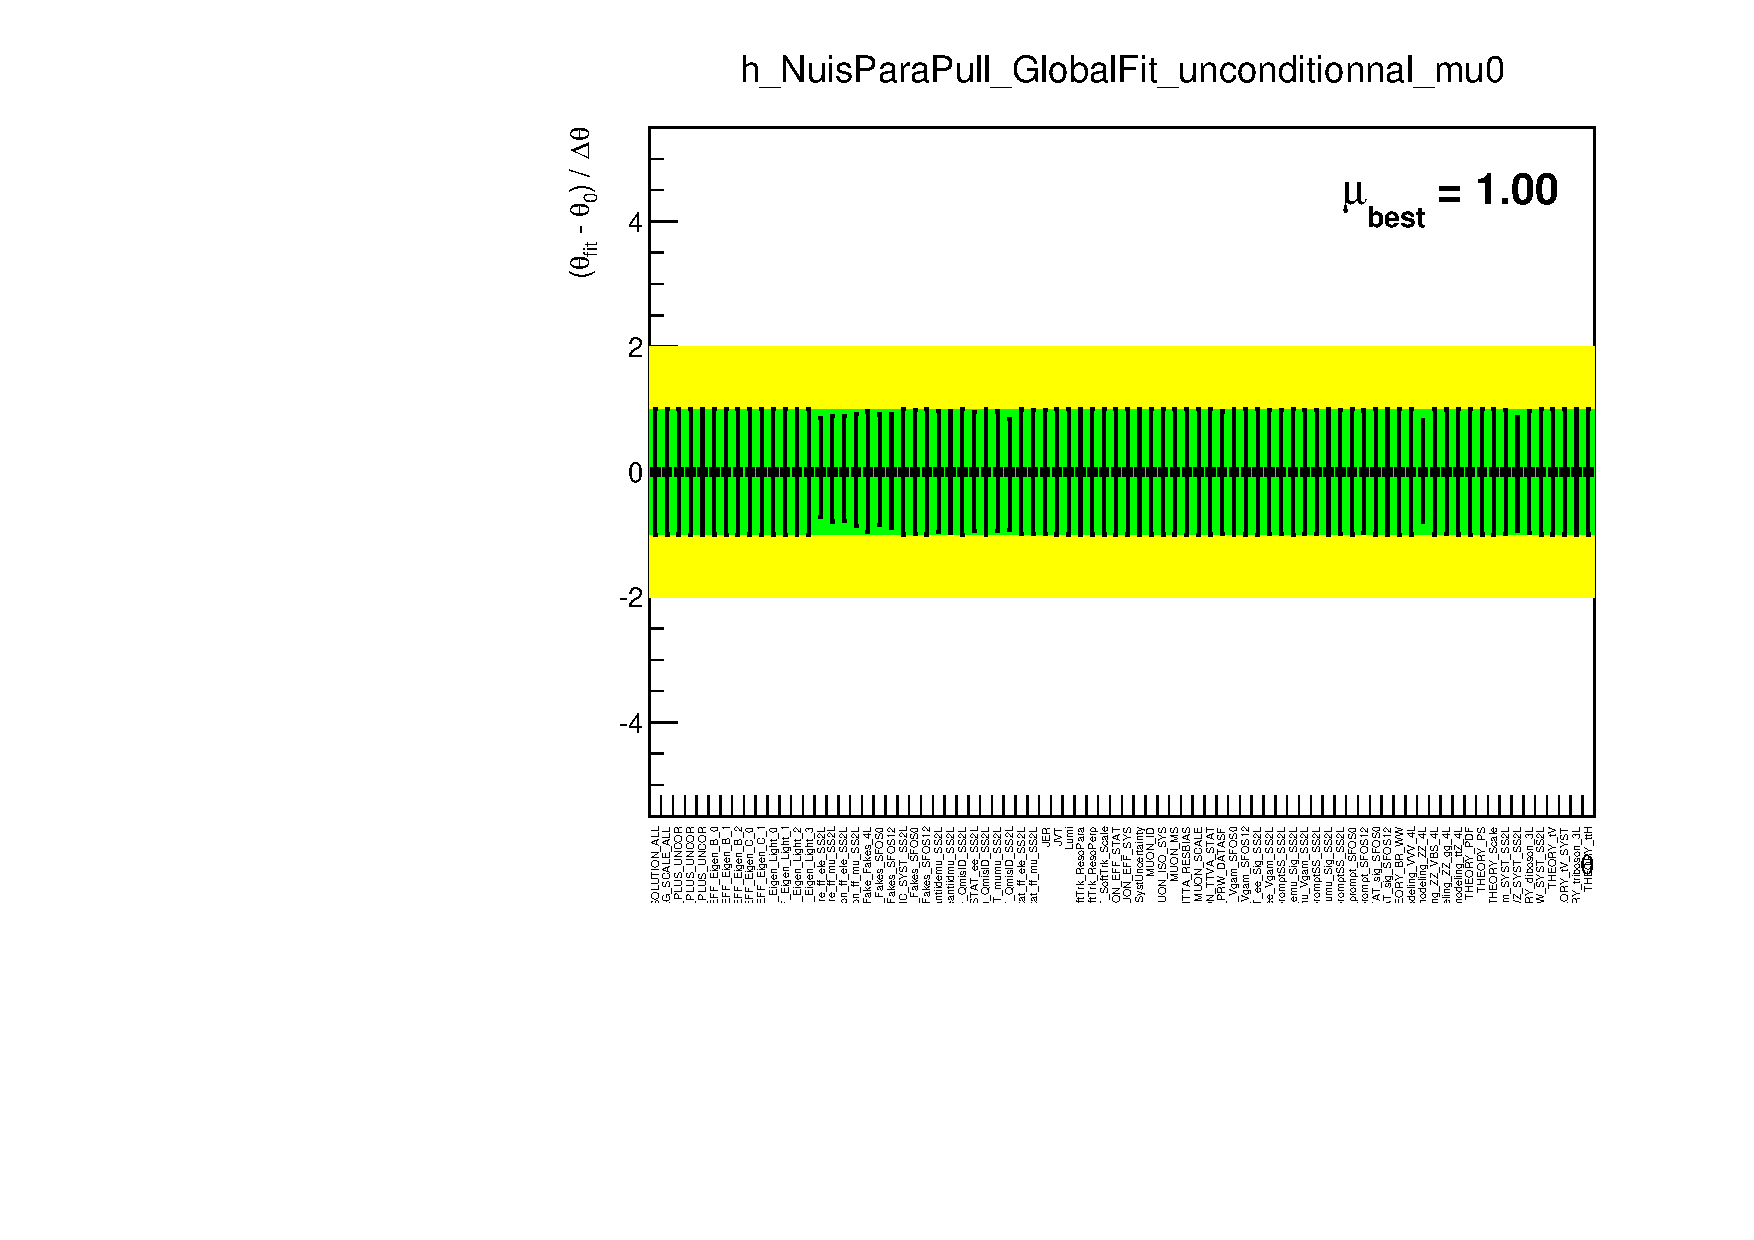
\includegraphics[width=.35\textwidth, angle=-90]{fig/Statistical/combination/pull-exp-combined-mH260_1_mu1.pdf}
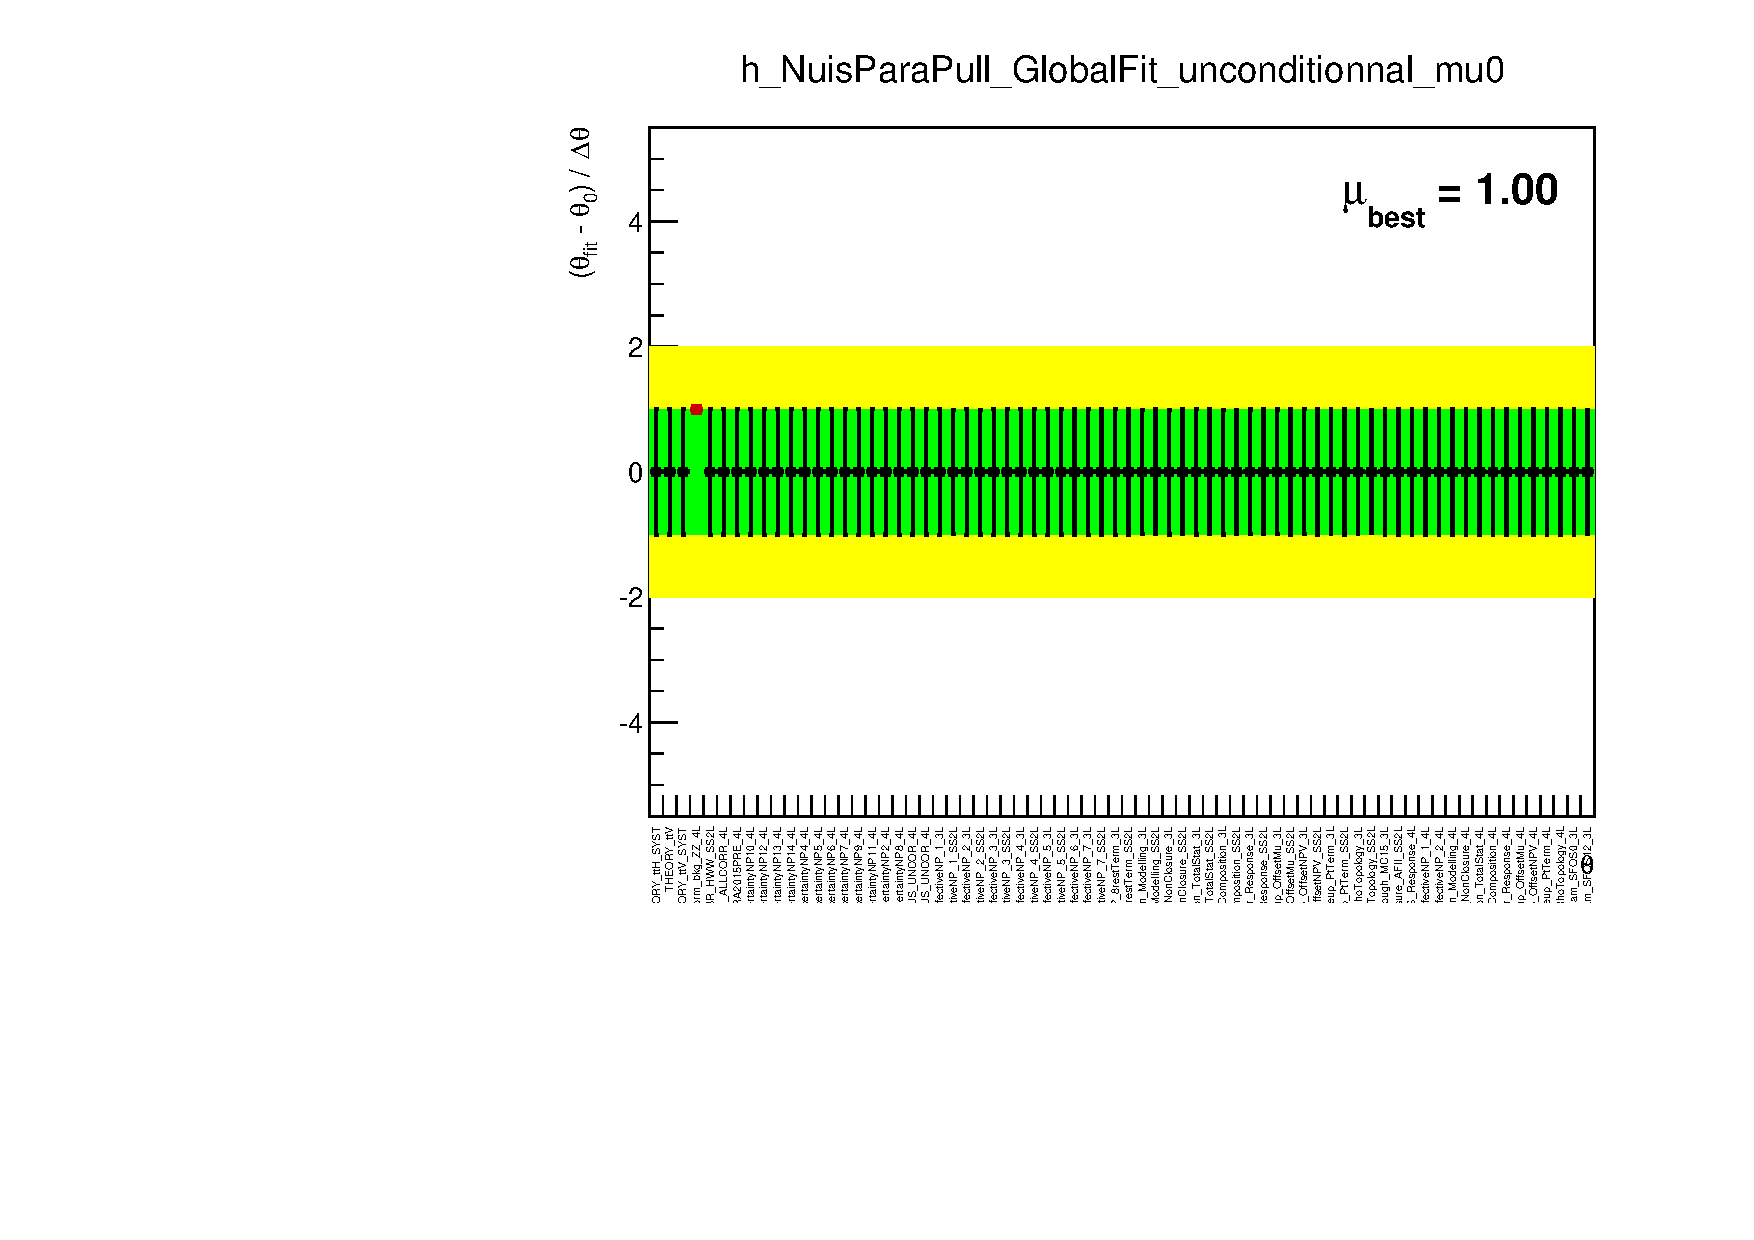
\includegraphics[width=.35\textwidth, angle=-90]{fig/Statistical/combination/pull-exp-combined-mH260_2_mu1.pdf}
\caption{S+B Asimov数据给出的$m_X$=260 GeV pull图。}
\label{fig:pull-exp-comb-260_mu1}
\end{figure}

\begin{figure}
\centering
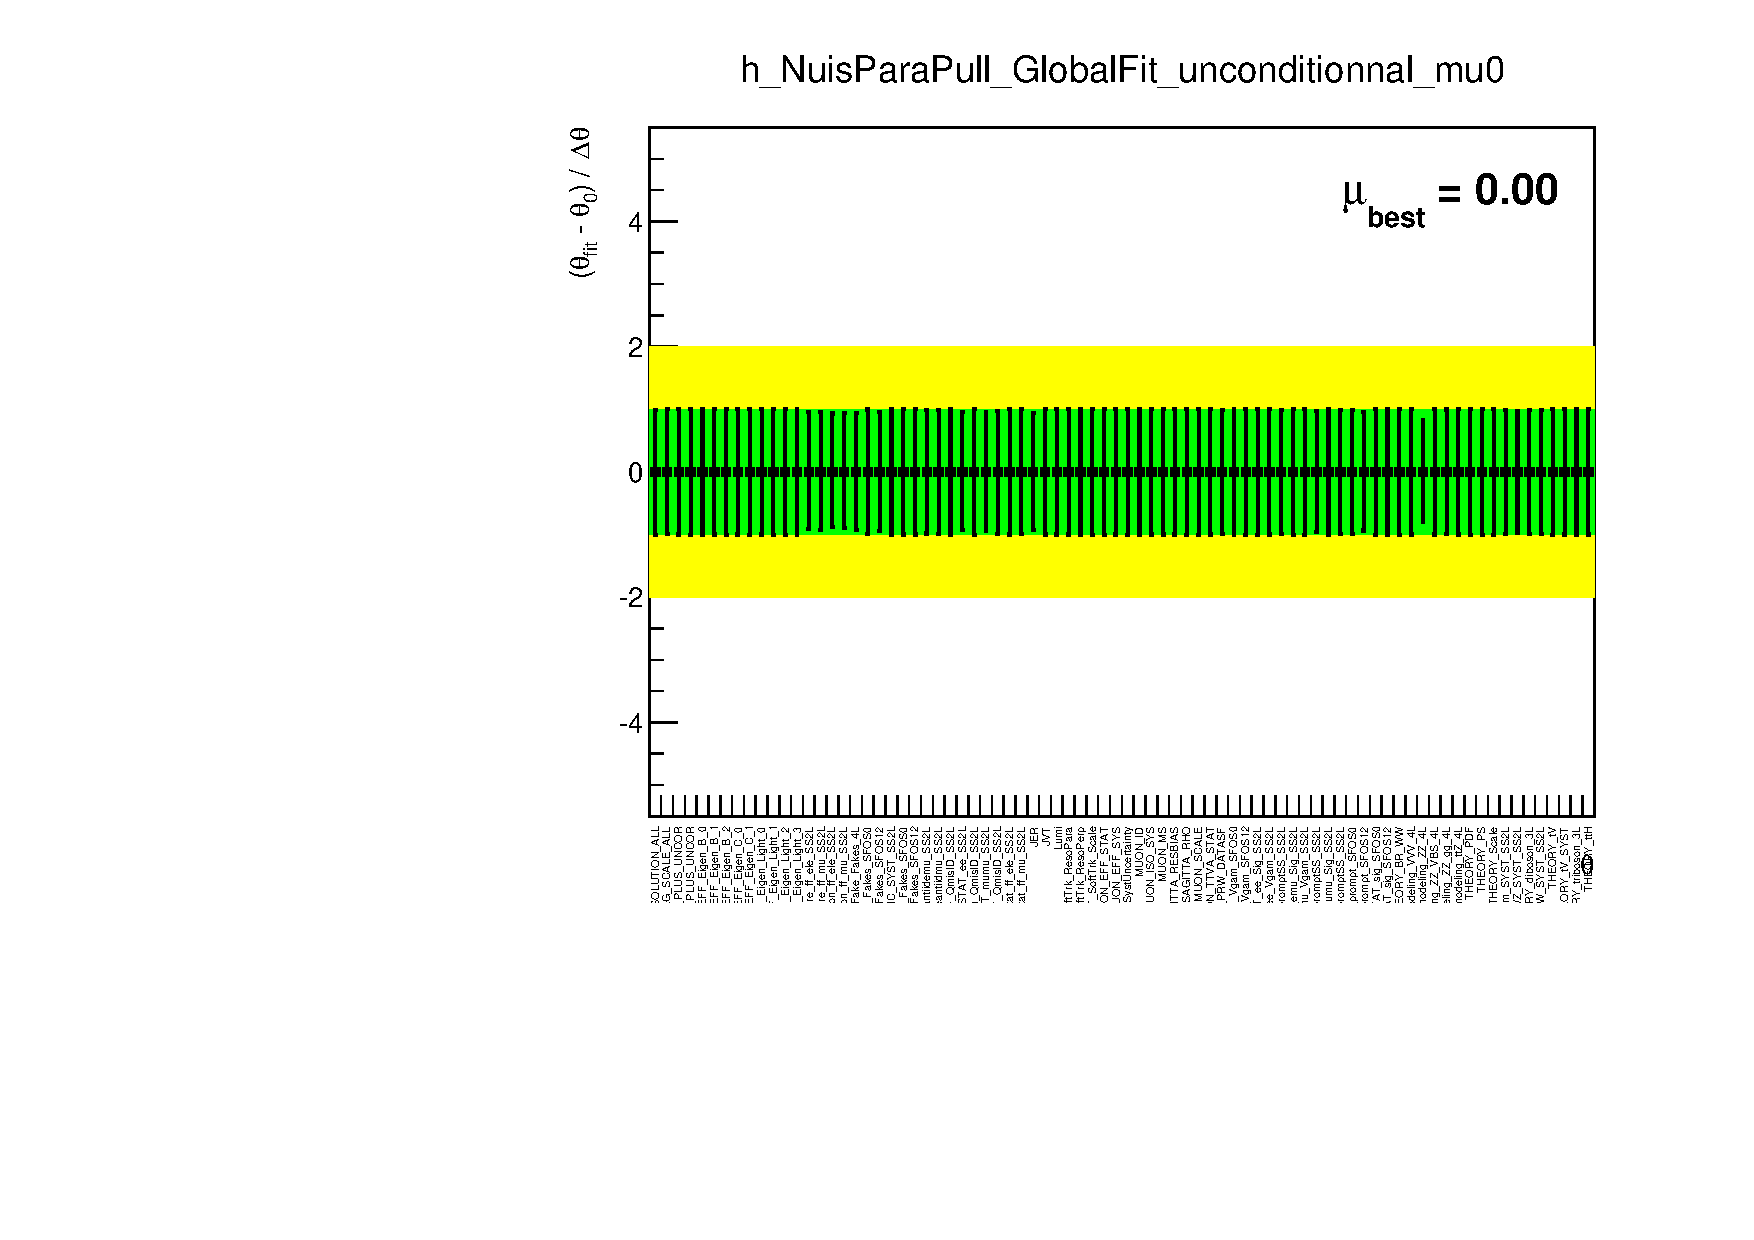
\includegraphics[width=.35\textwidth, angle=-90]{fig/Statistical/combination/pull-exp-combined-mH500_1.pdf}
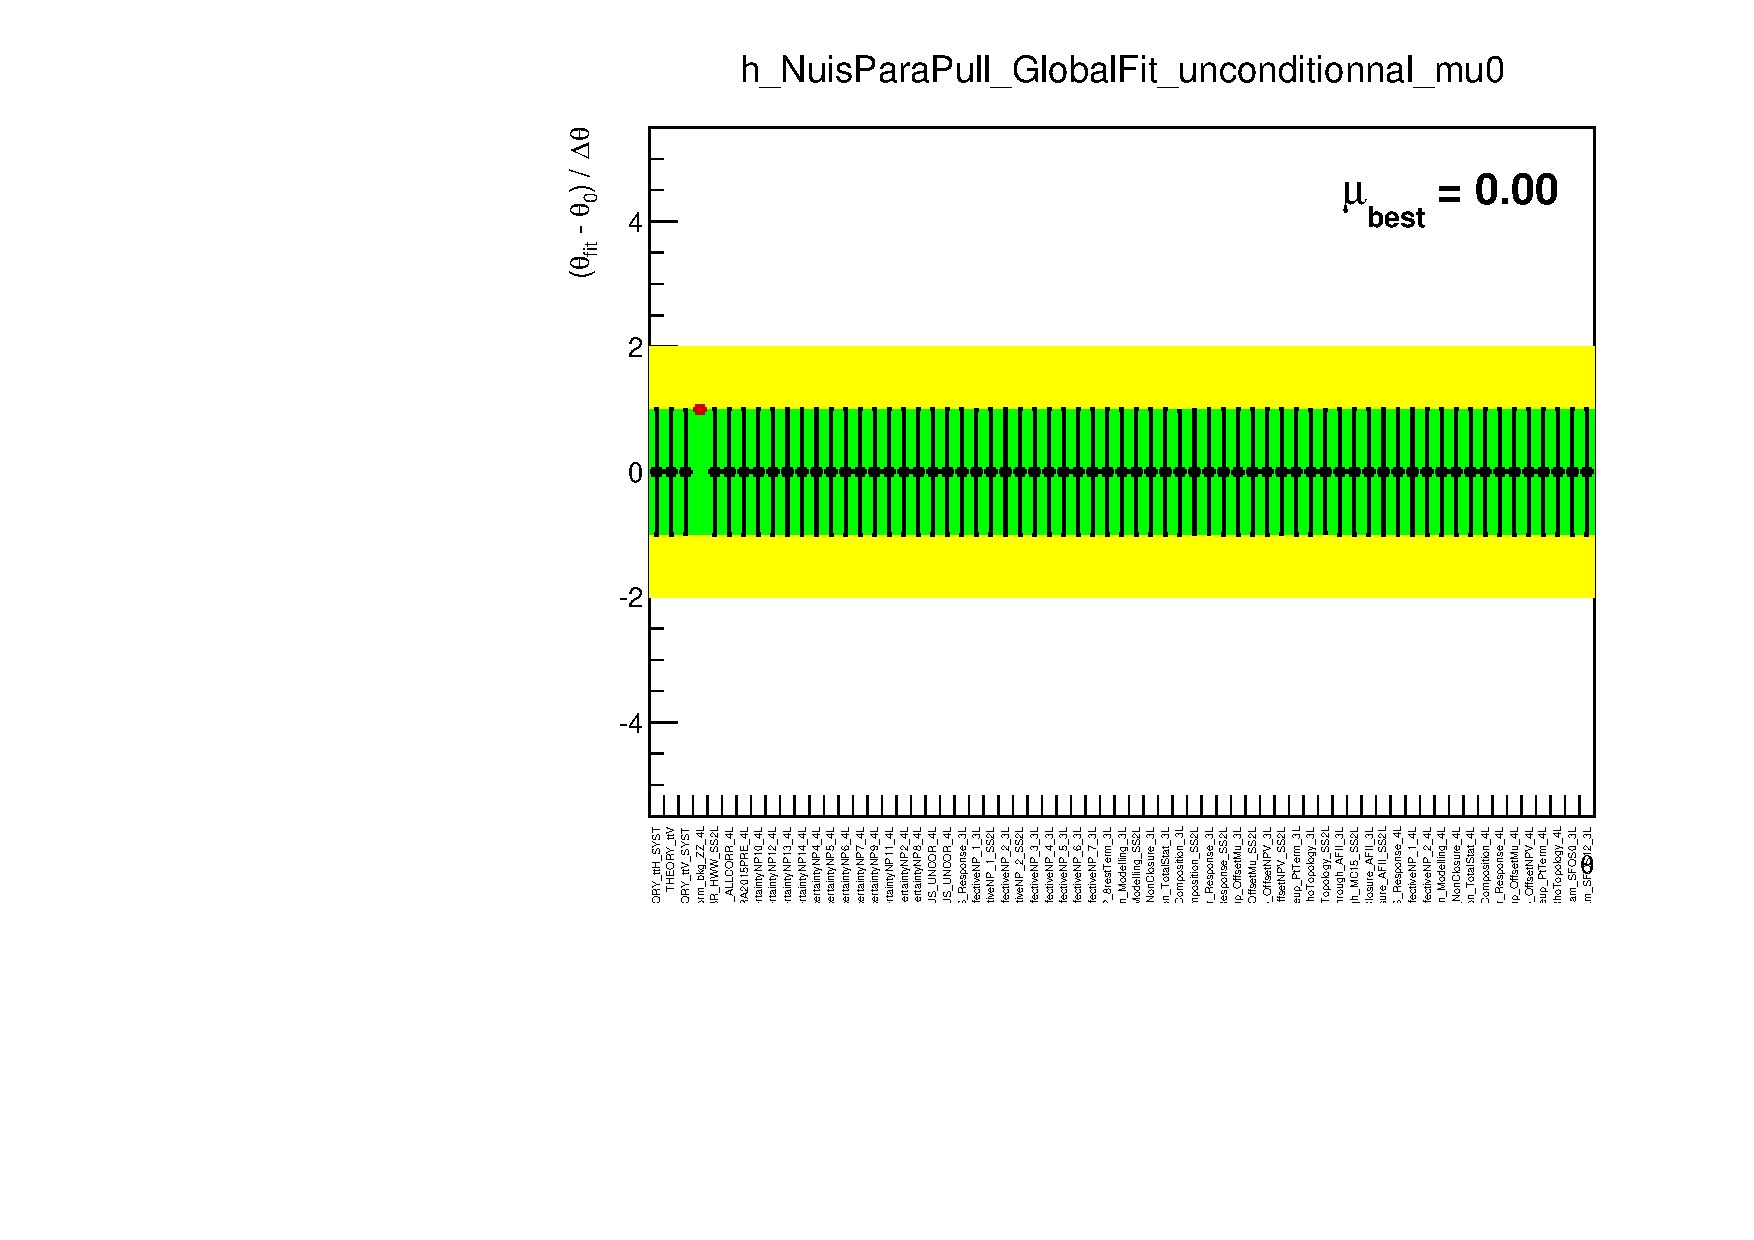
\includegraphics[width=.35\textwidth, angle=-90]{fig/Statistical/combination/pull-exp-combined-mH500_2.pdf}
%\caption{pull check on B-only asimovData of $m_{H}=500 GeV$}
\caption{无信号Asimov数据给出的$m_X$=500 GeV pull图。}
\label{fig:pull-exp-comb-500}
\end{figure}

\begin{figure}
\centering
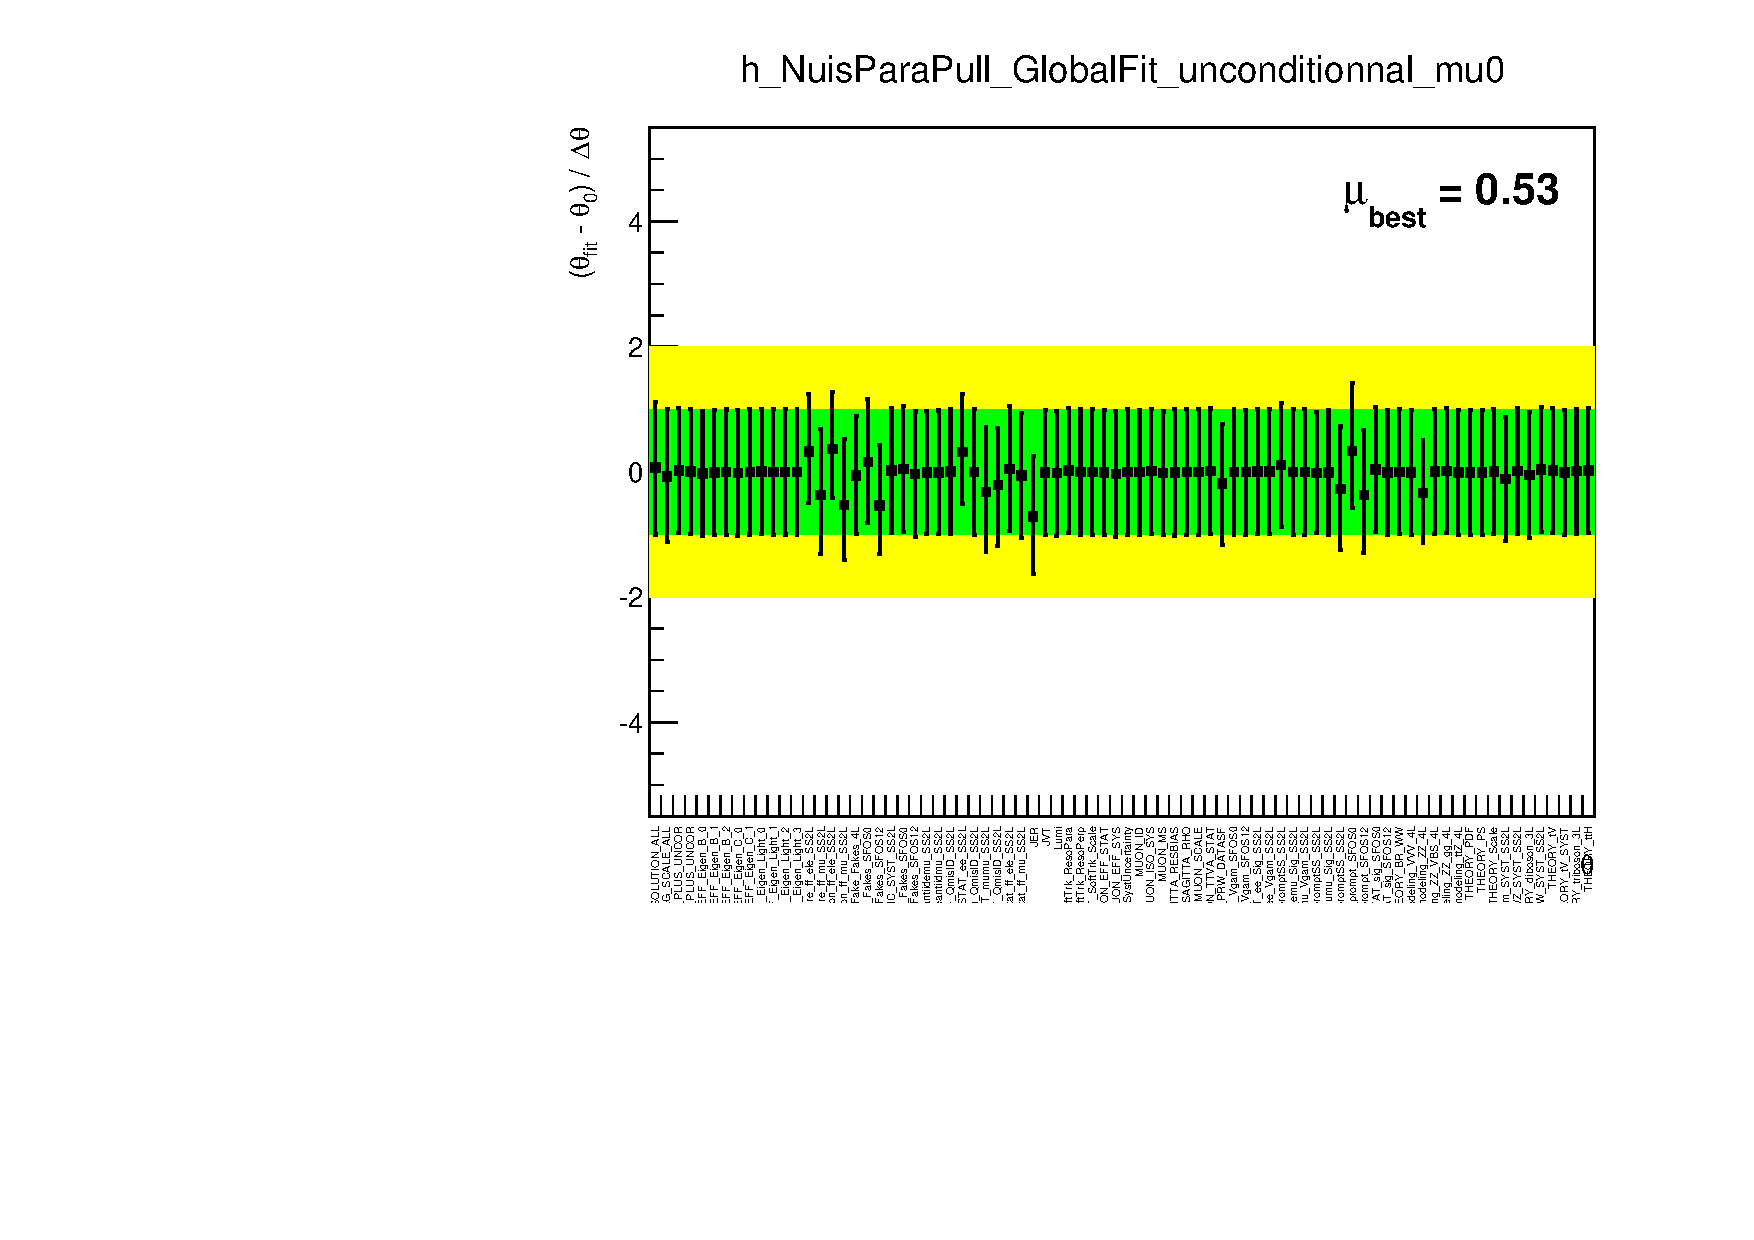
\includegraphics[width=.35\textwidth, angle=-90]{fig/Statistical/combination/pull-obs-combined-mH500_1.pdf}
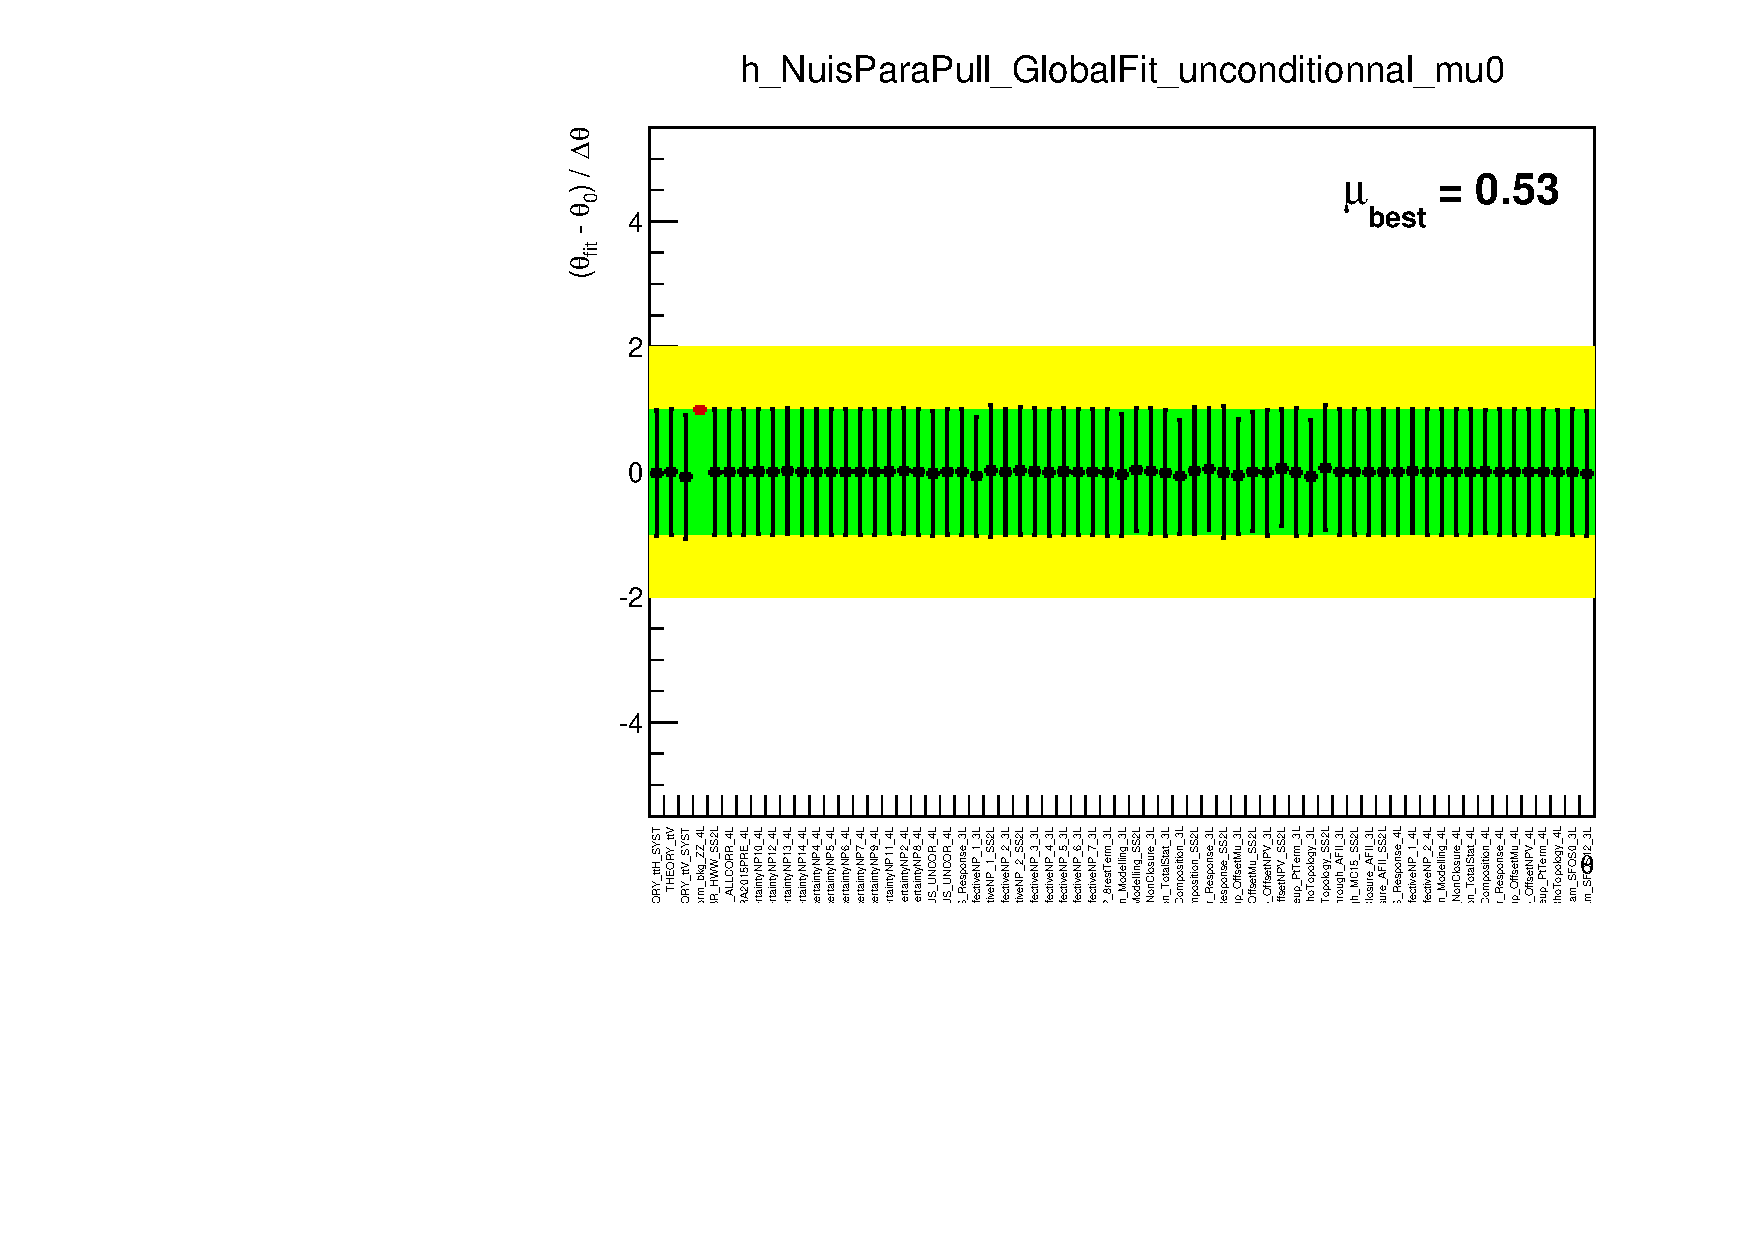
\includegraphics[width=.35\textwidth, angle=-90]{fig/Statistical/combination/pull-obs-combined-mH500_2.pdf}
%\caption{pull check on obsData of $m_{H}=500 GeV$}
\caption{观测数据给出的$m_X$=500 GeV pull图。}
\label{fig:pull-obs-comb-500}
\end{figure}

\begin{figure}
\centering
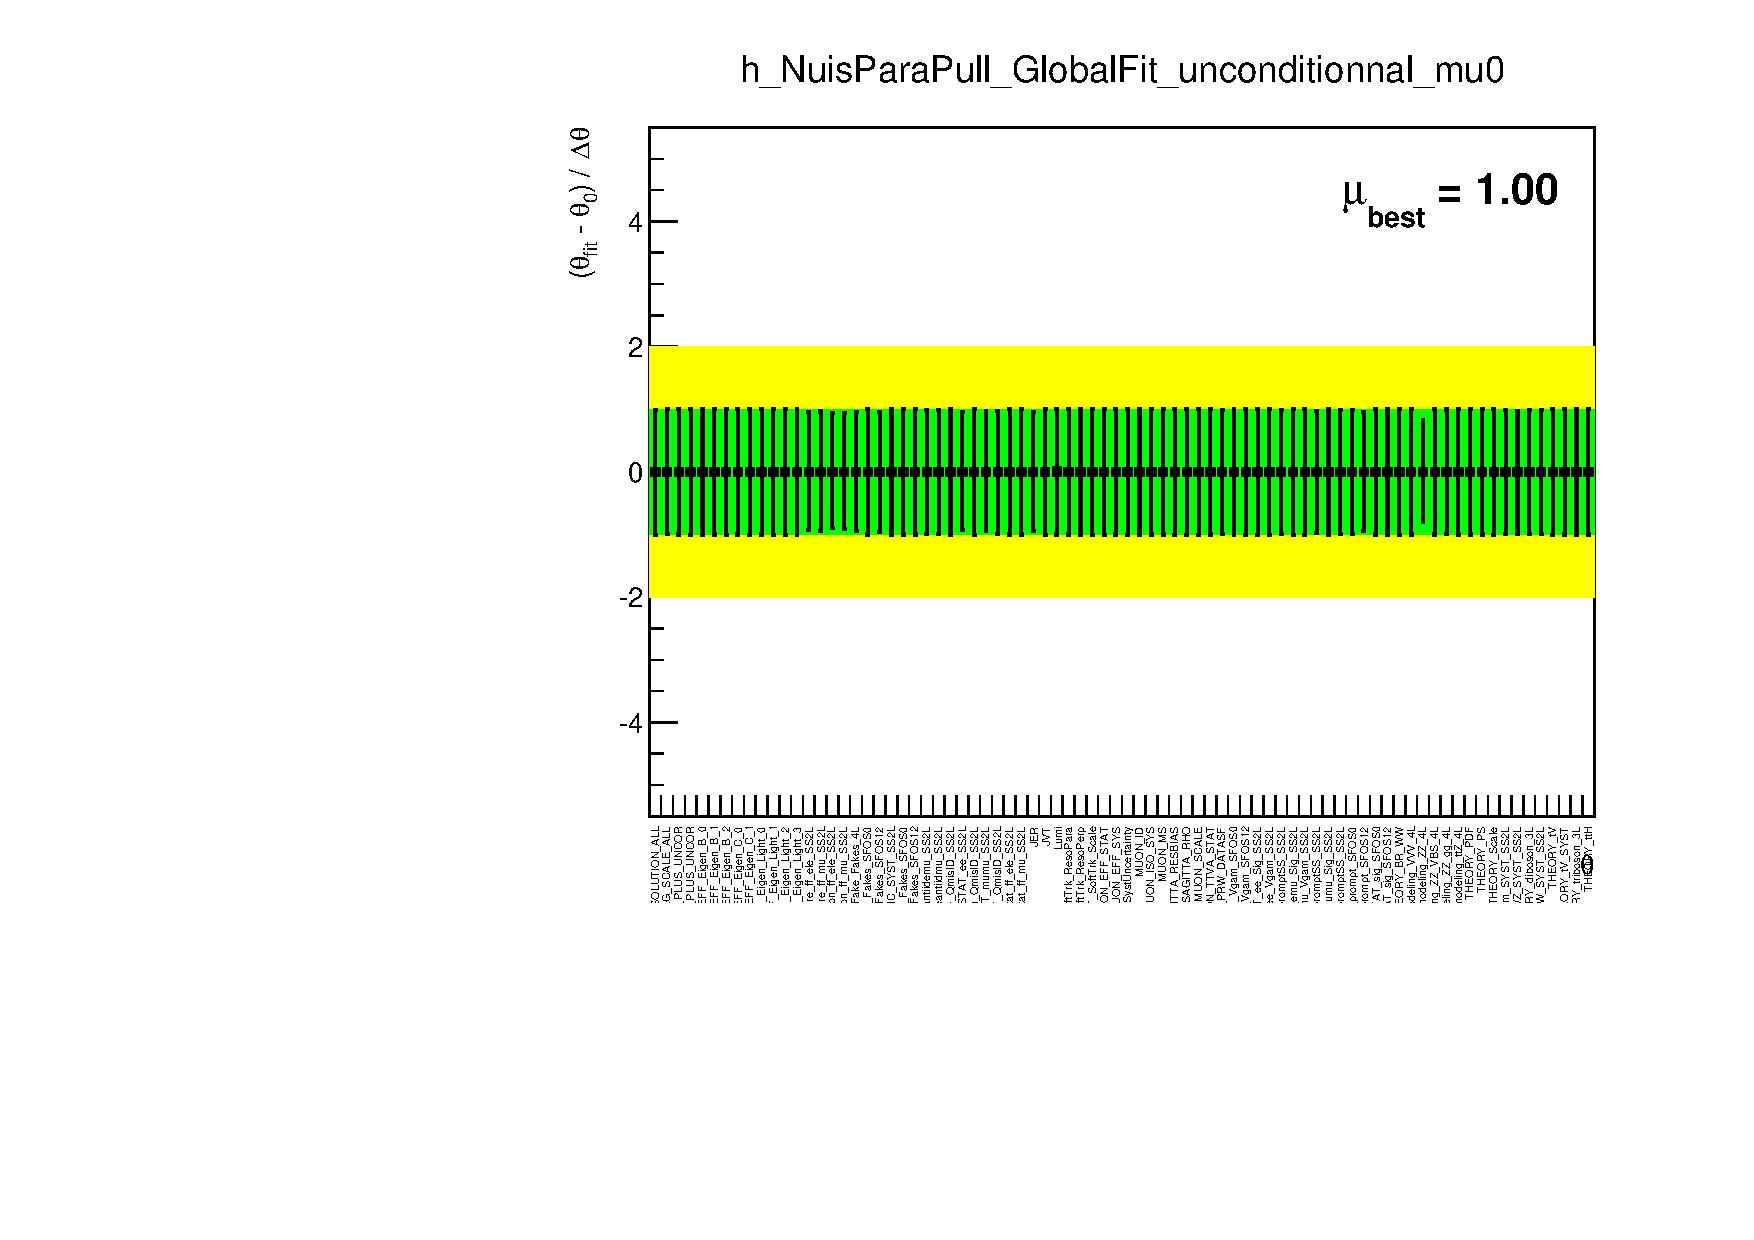
\includegraphics[width=.35\textwidth, angle=-90]{fig/Statistical/combination/pull-exp-combined-mH500_1_mu1.pdf}
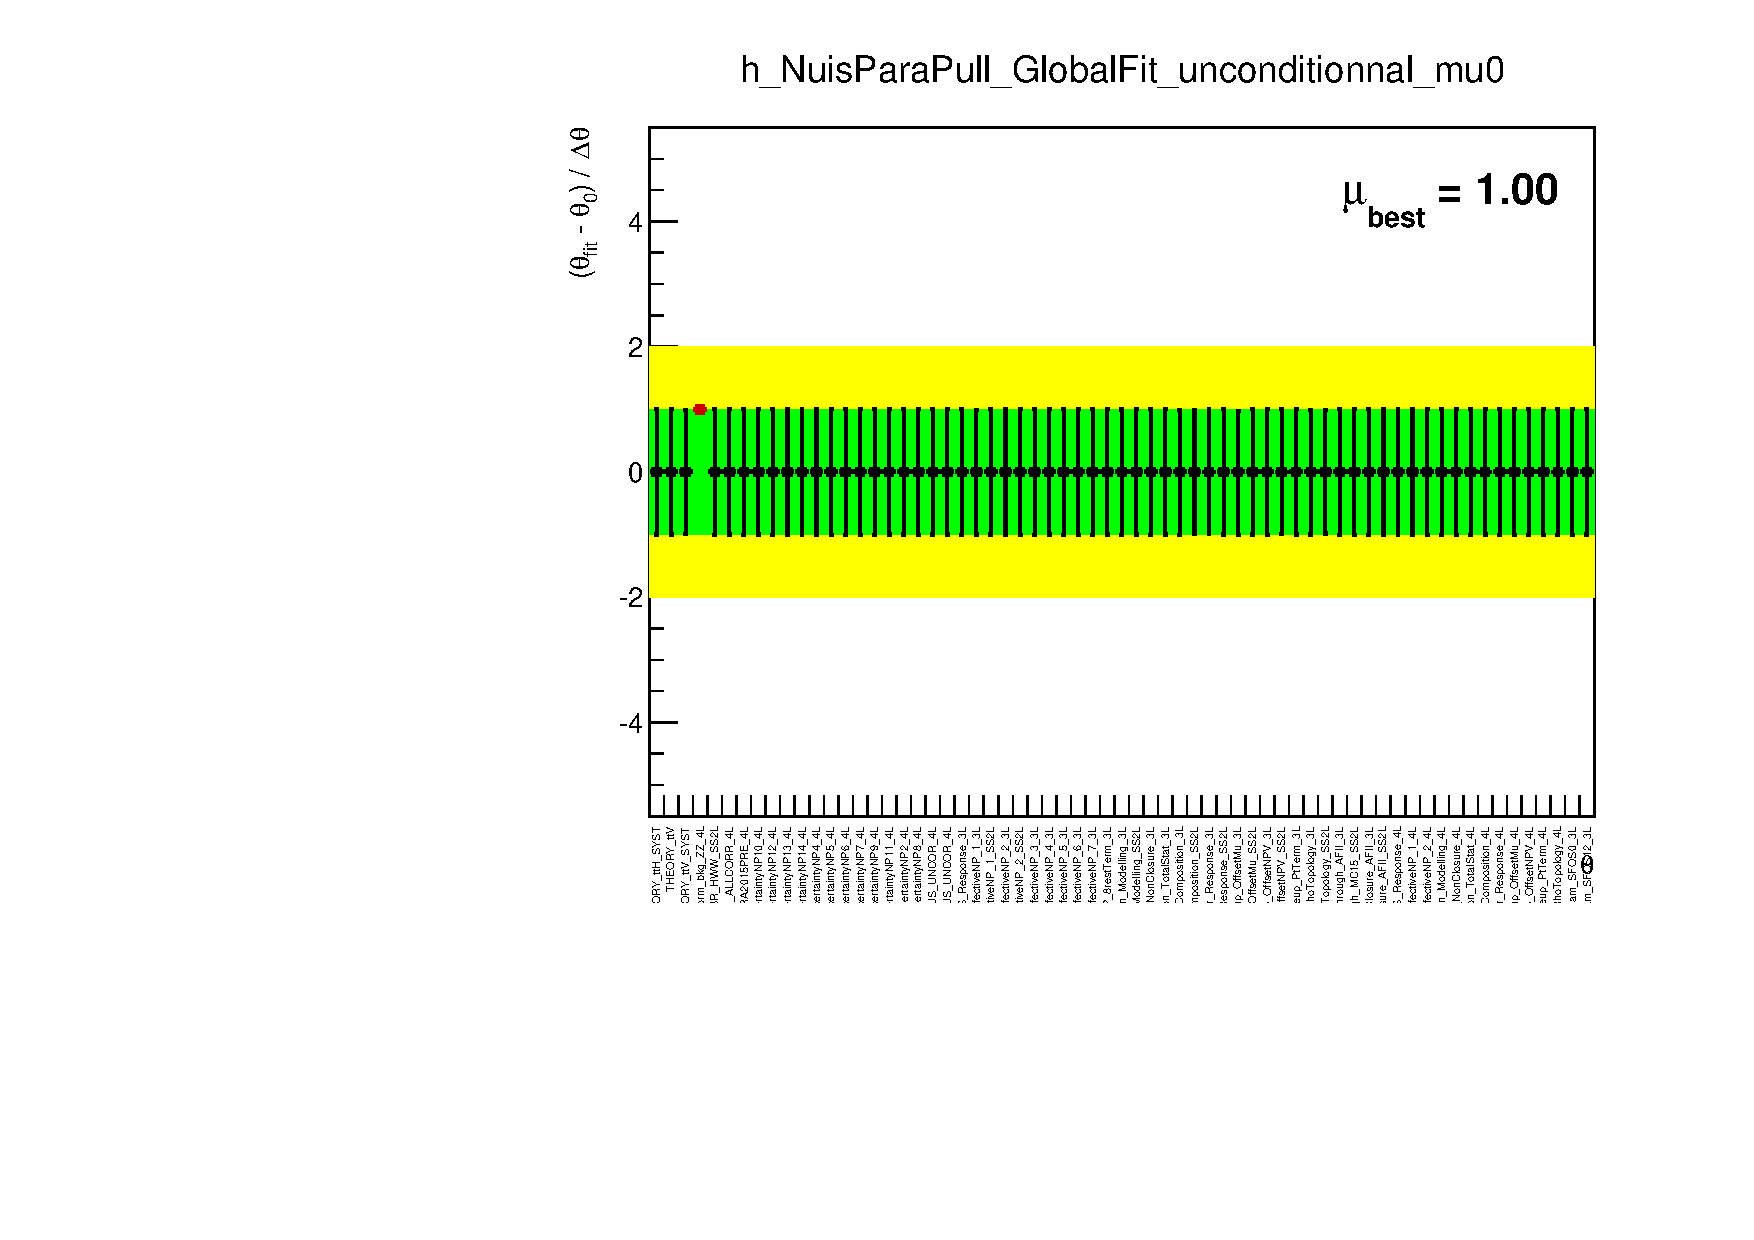
\includegraphics[width=.35\textwidth, angle=-90]{fig/Statistical/combination/pull-exp-combined-mH500_2_mu1.pdf}
%\caption{pull check on S+B asimovData of $m_{H}=500 GeV$}
\caption{S+B Asimov数据给出的$m_X$=500 GeV pull图。}
\label{fig:pull-exp-comb-500_mu1}
\end{figure}

\begin{figure}
\centering
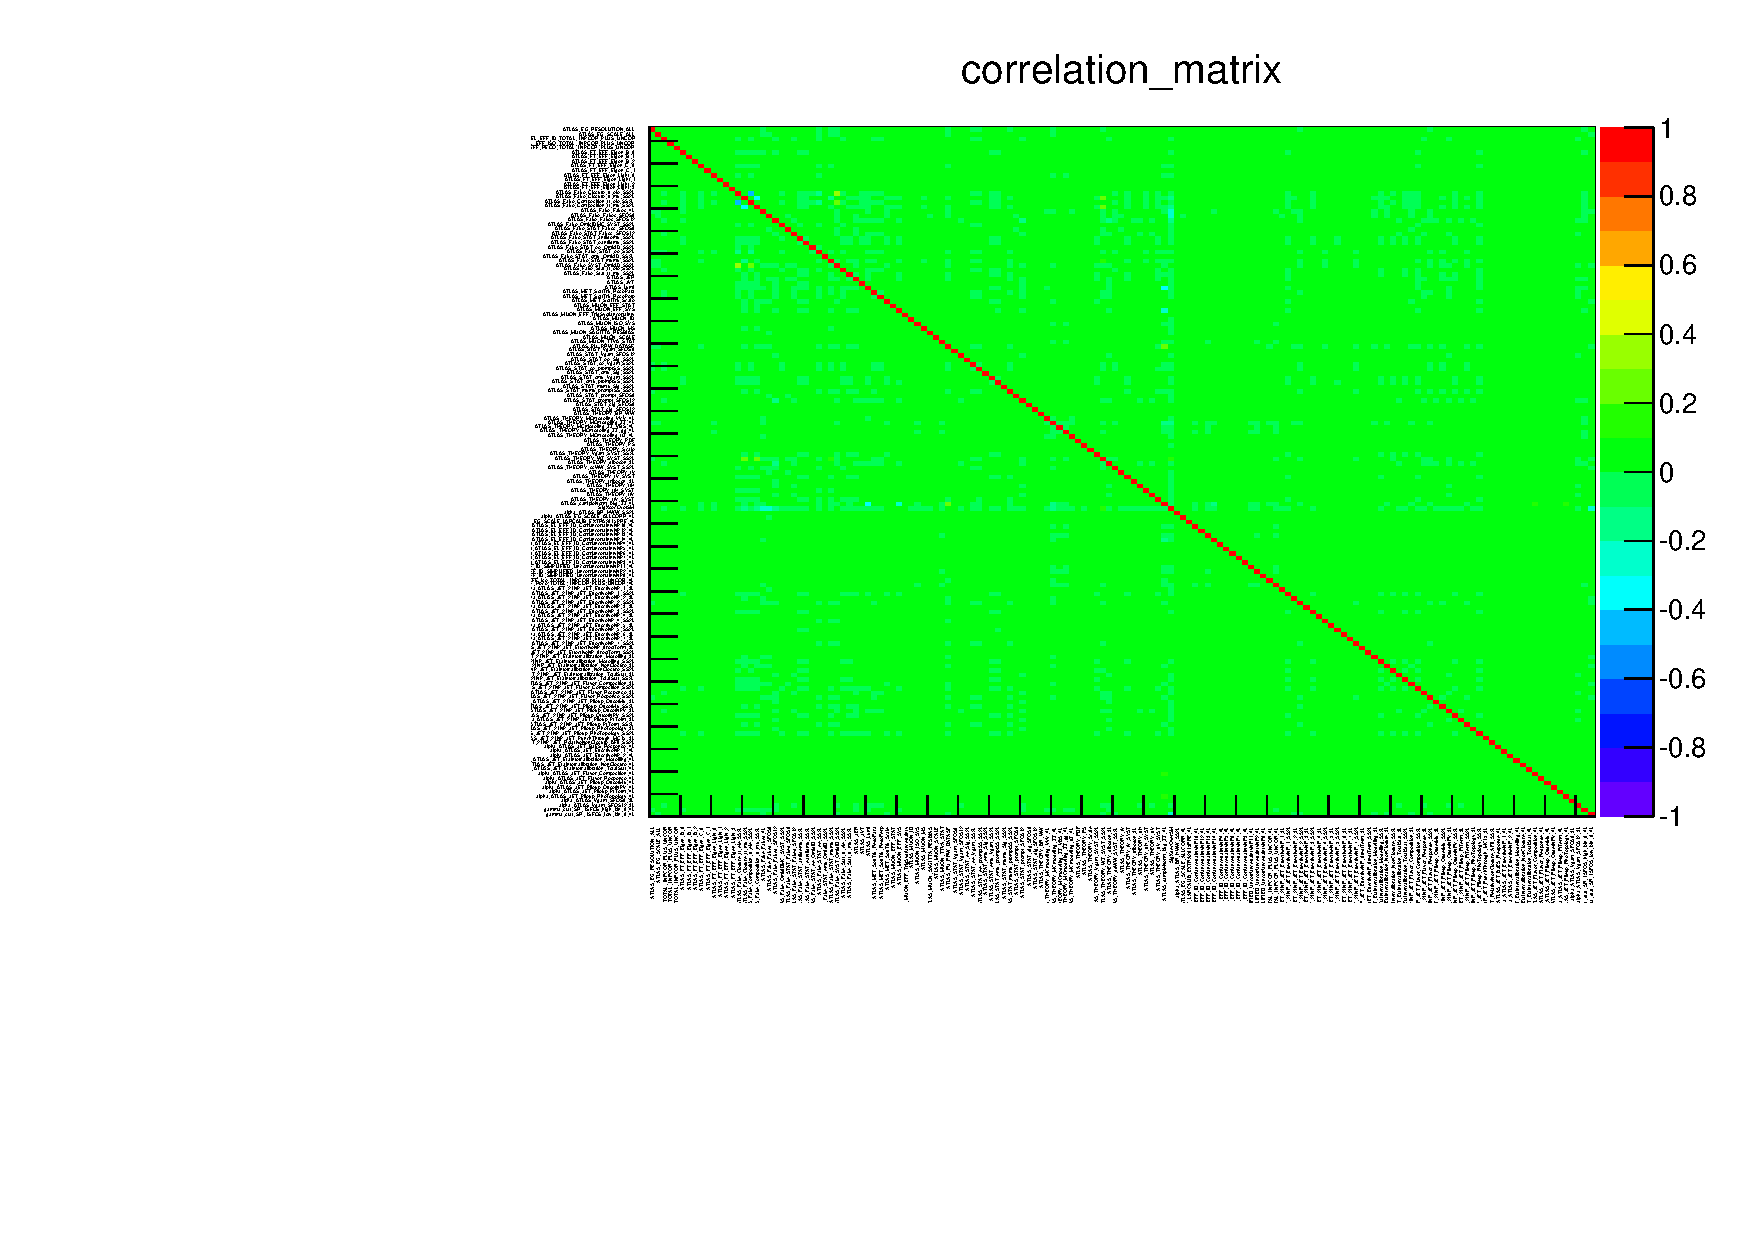
\includegraphics[width=.35\textwidth, angle=-90]{fig/Statistical/combination/corr-exp-combined-mH260.pdf}
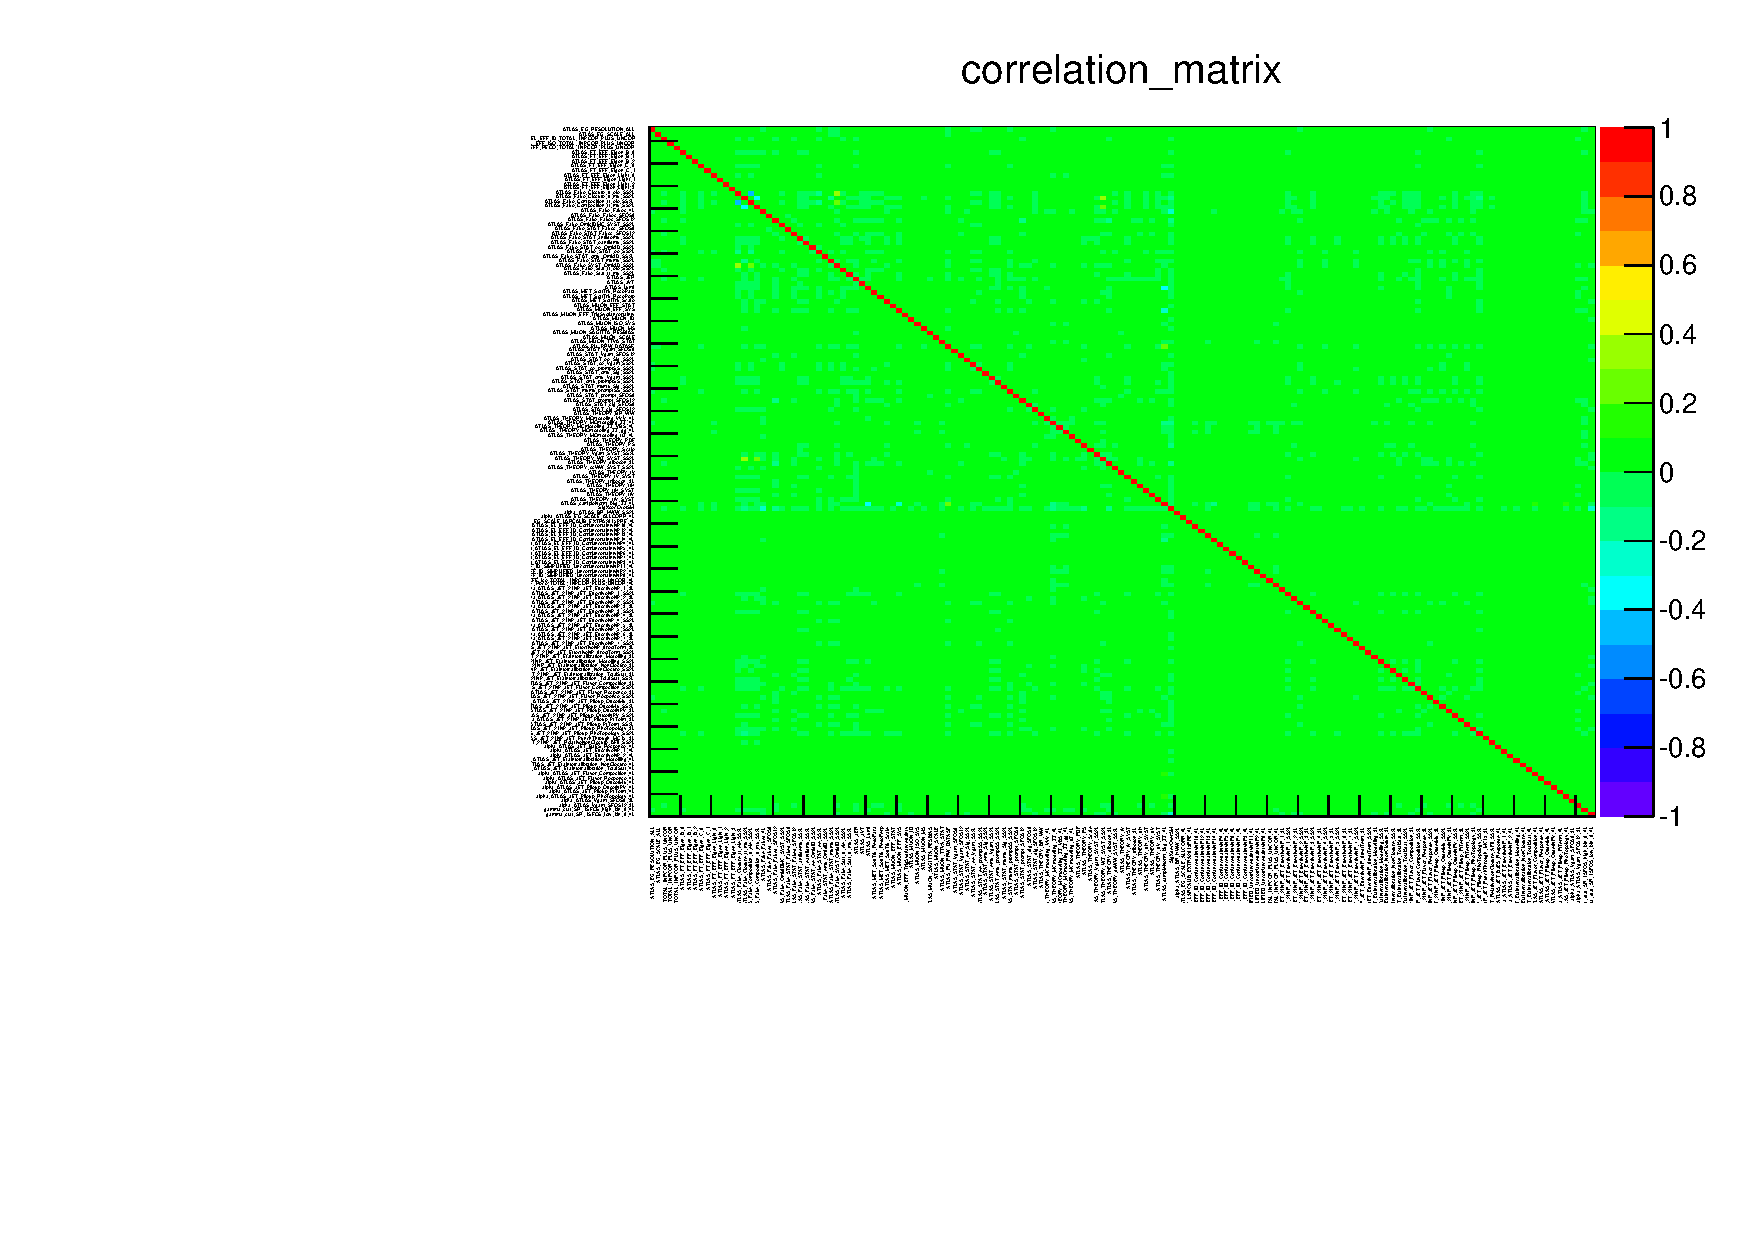
\includegraphics[width=.35\textwidth, angle=-90]{fig/Statistical/combination/corr-obs-combined-mH260.pdf}\\
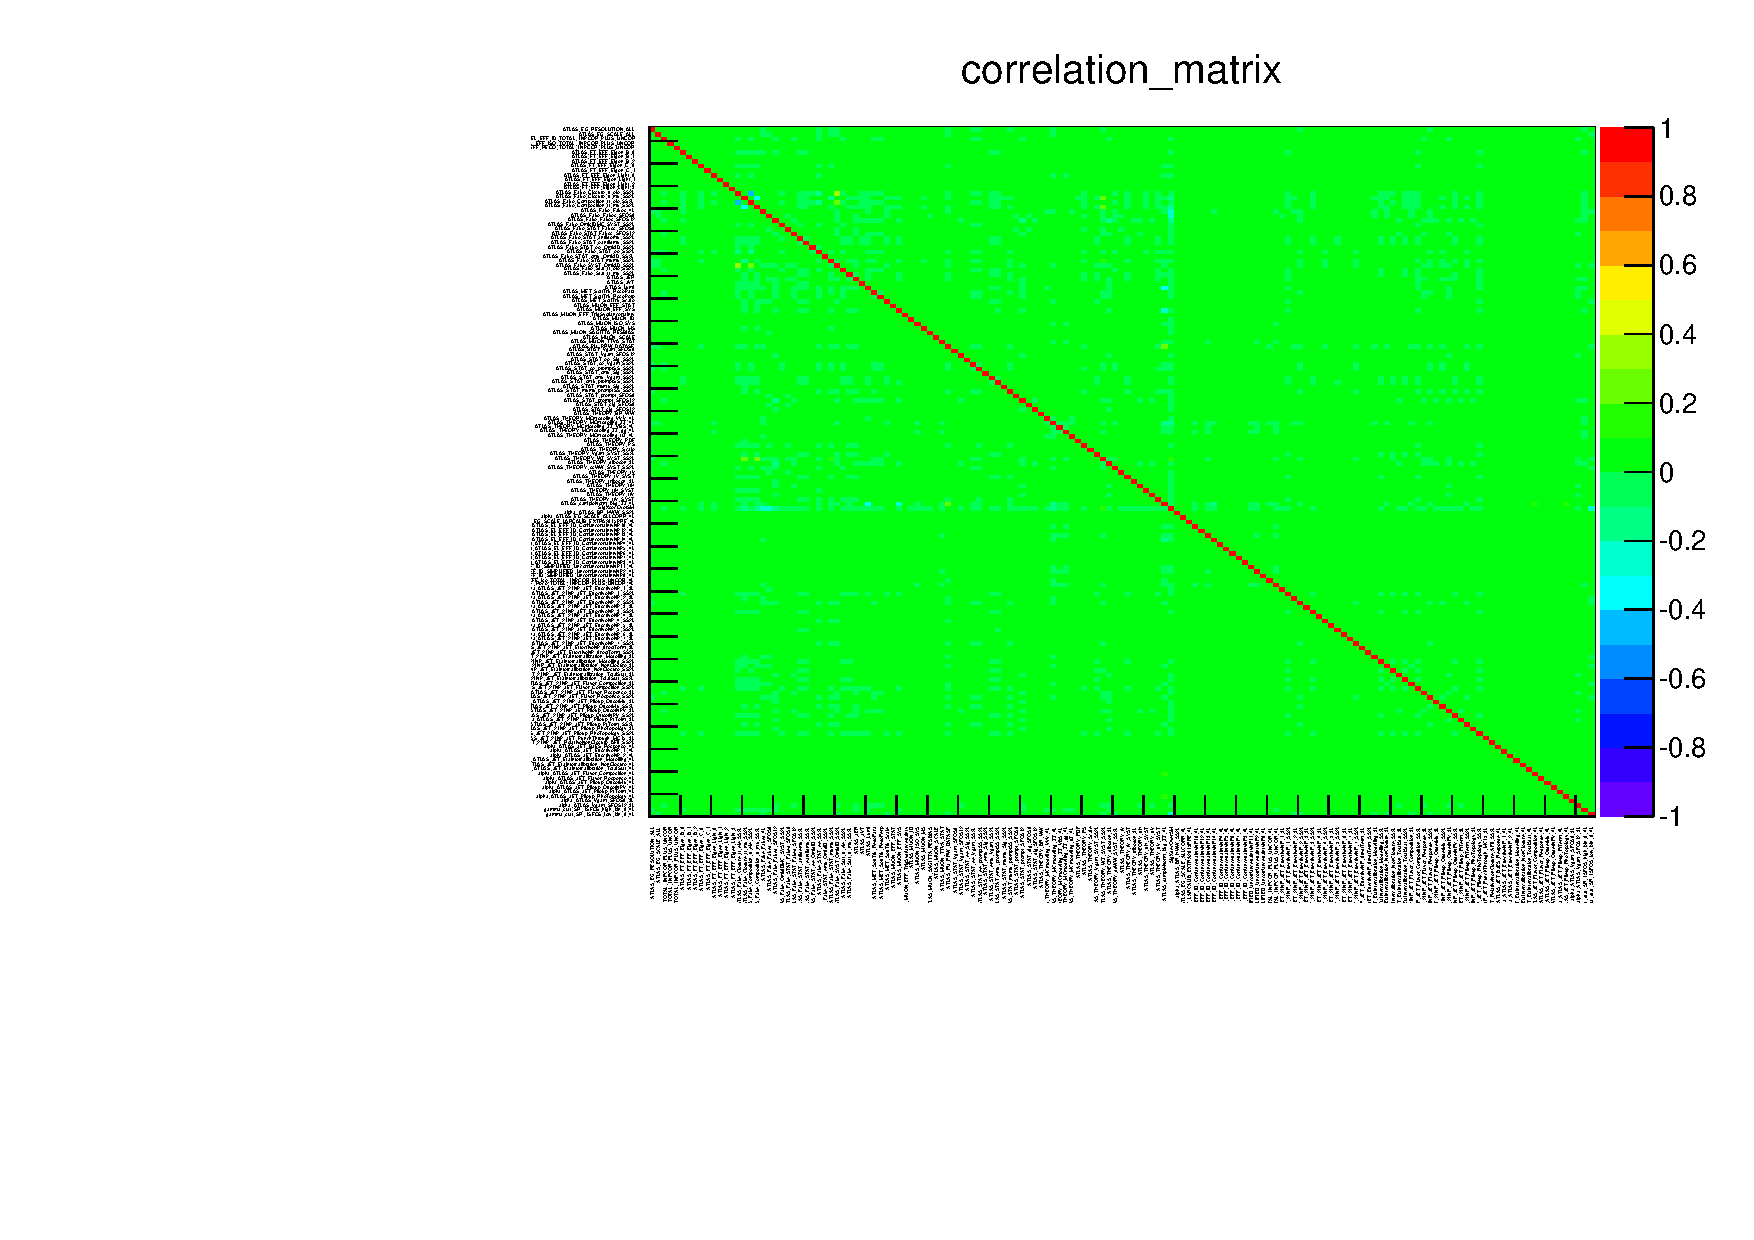
\includegraphics[width=.35\textwidth, angle=-90]{fig/Statistical/combination/corr-exp-combined-mH260_mu1.pdf}
%\caption{correlation check on B-only asimovData, obsData and S+B asimovData of $m_{H}=260 GeV$}
\caption{$m_X$=260 GeV分析NP相关性检查,分别对应无信号Asimov数据,观测数据和S+B Asimov数据。}
\label{fig:corr-comb-260}
\end{figure}

\begin{figure}
\centering
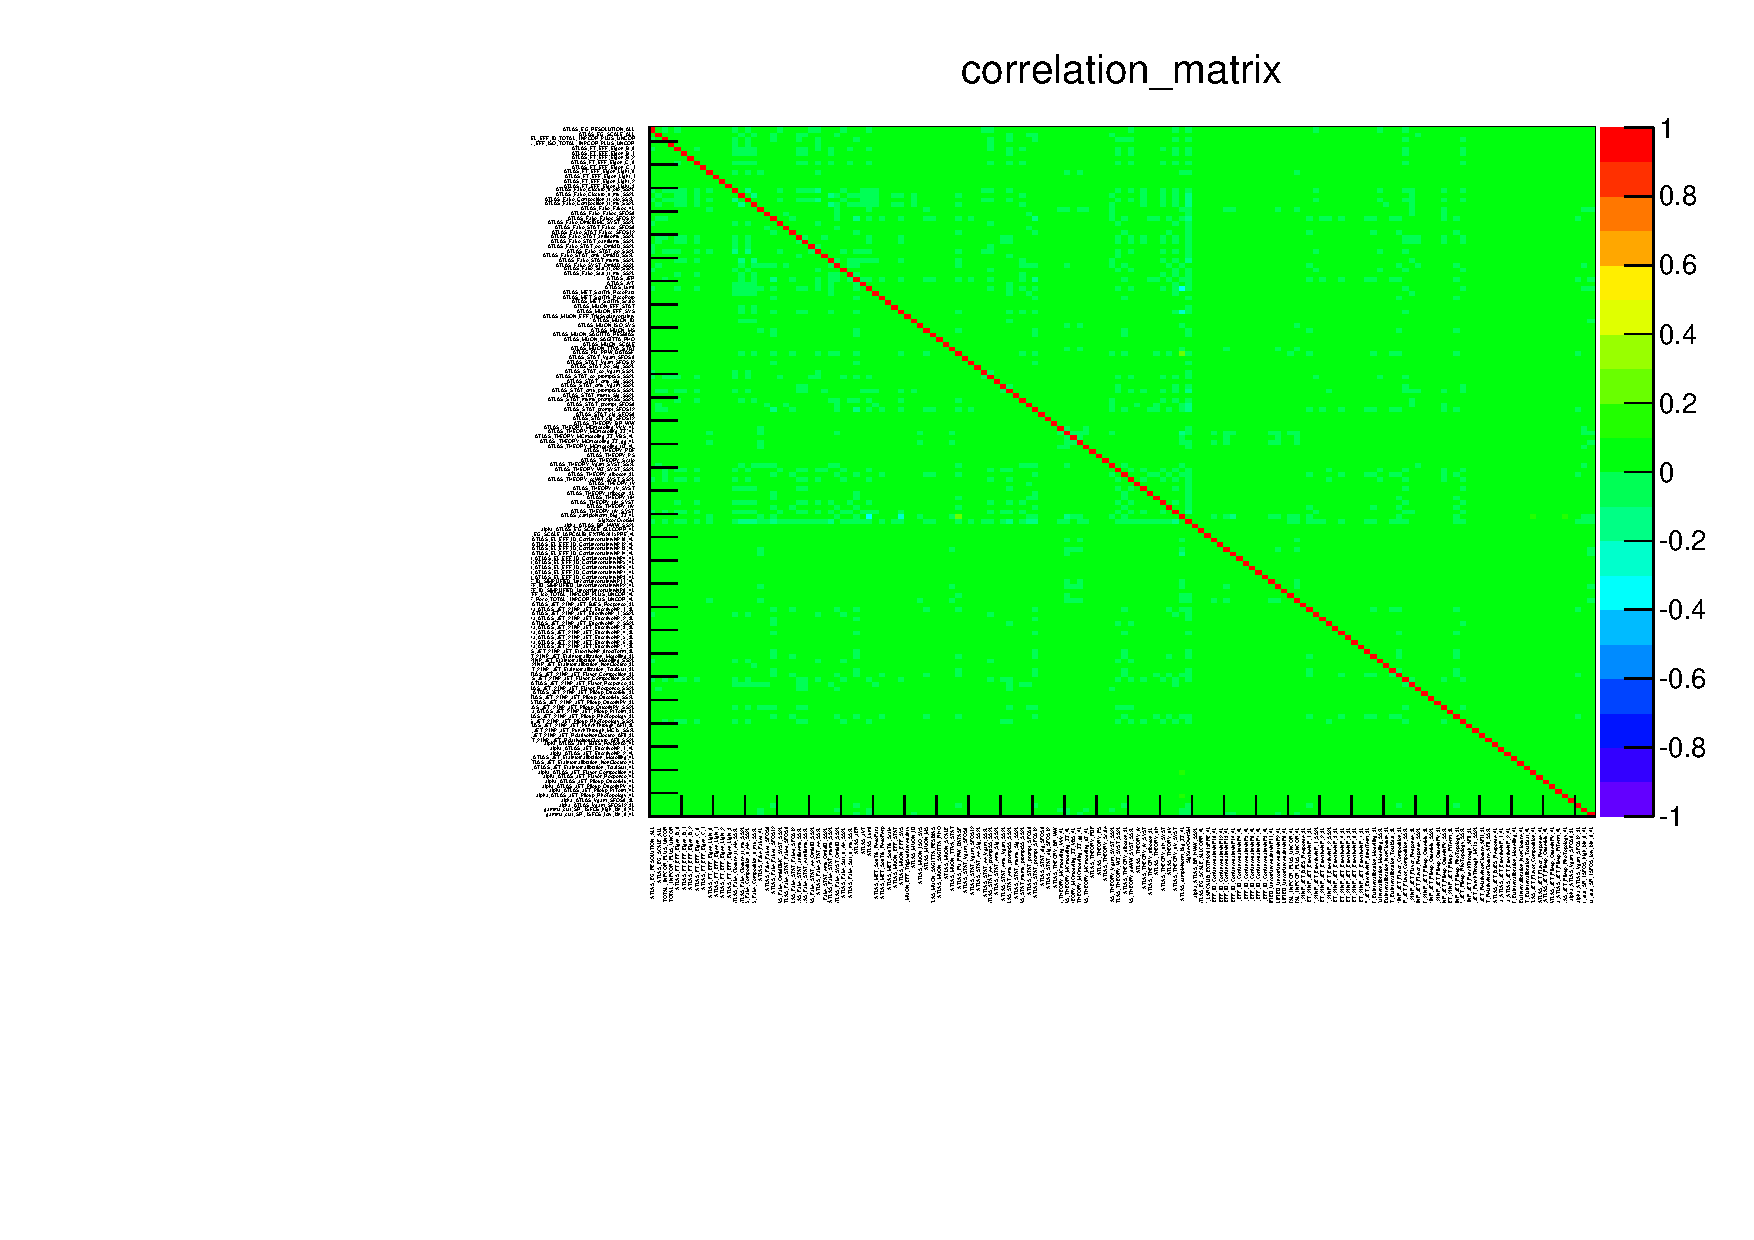
\includegraphics[width=.35\textwidth, angle=-90]{fig/Statistical/combination/corr-exp-combined-mH500.pdf}
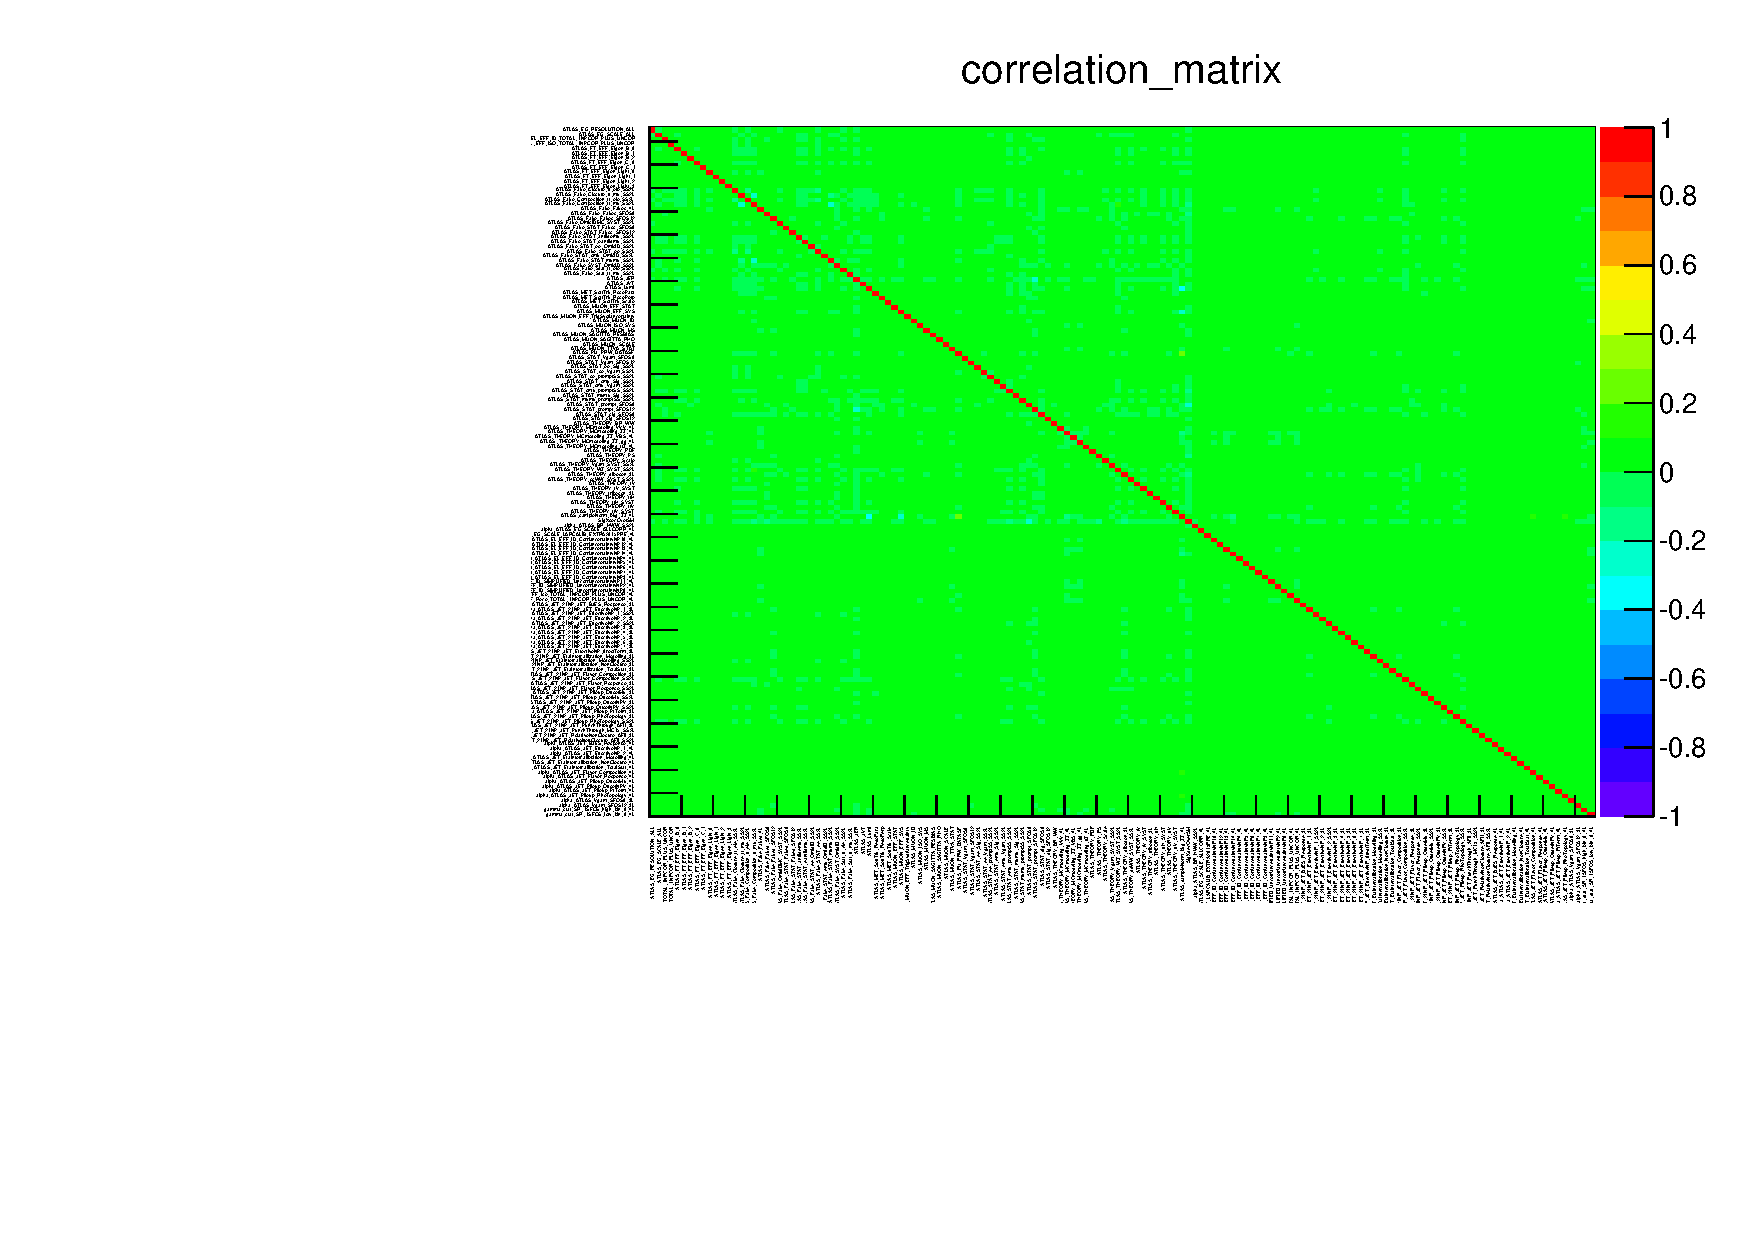
\includegraphics[width=.35\textwidth, angle=-90]{fig/Statistical/combination/corr-obs-combined-mH500.pdf}\\
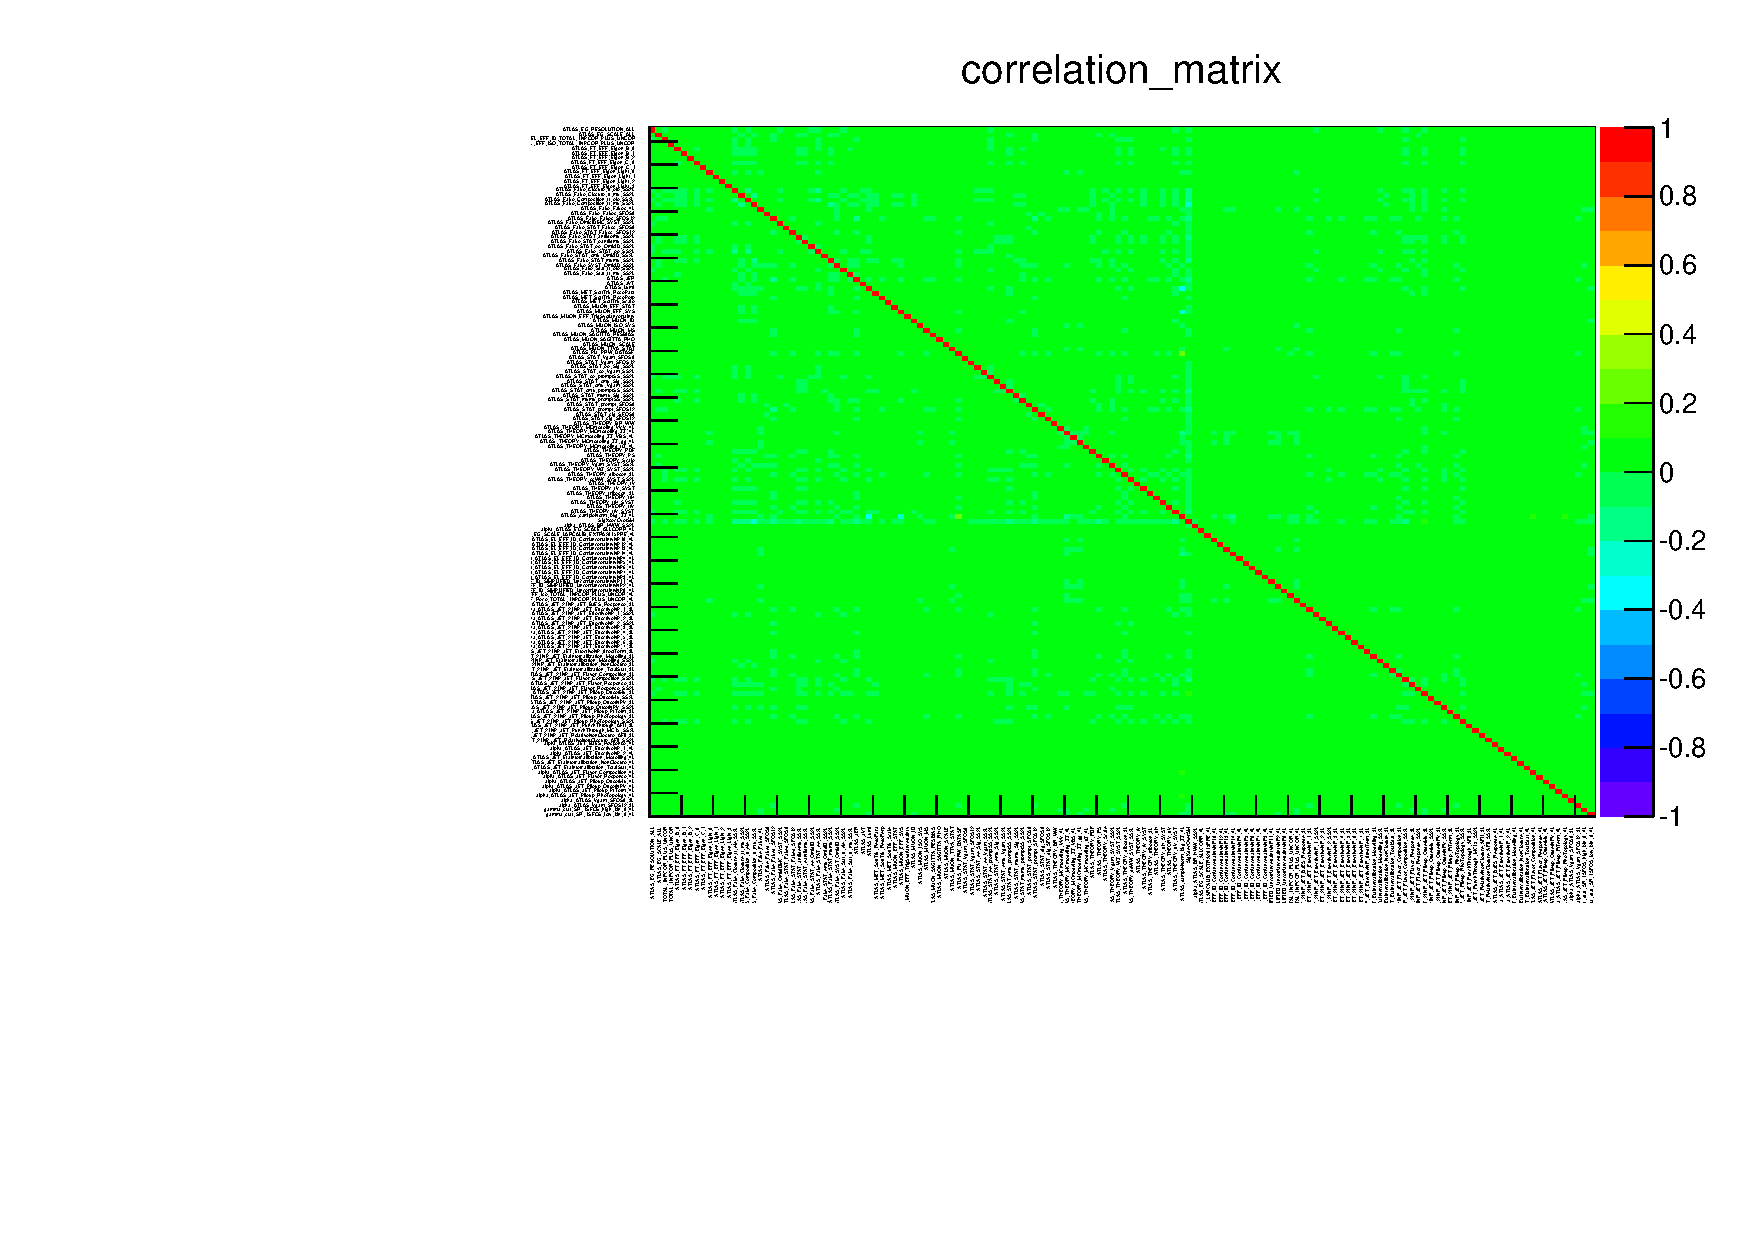
\includegraphics[width=.35\textwidth, angle=-90]{fig/Statistical/combination/corr-exp-combined-mH500_mu1.pdf}
%\caption{correlation check on B-only asimovData, obsData and S+B asimovData of $m_{H}=500 GeV$}
\caption{$m_X$=500 GeV分析NP相关性检查,分别对应无信号Asimov数据,观测数据和S+B Asimov数据。}
\label{fig:corr-comb-500}
\end{figure}

\begin{figure}
\centering
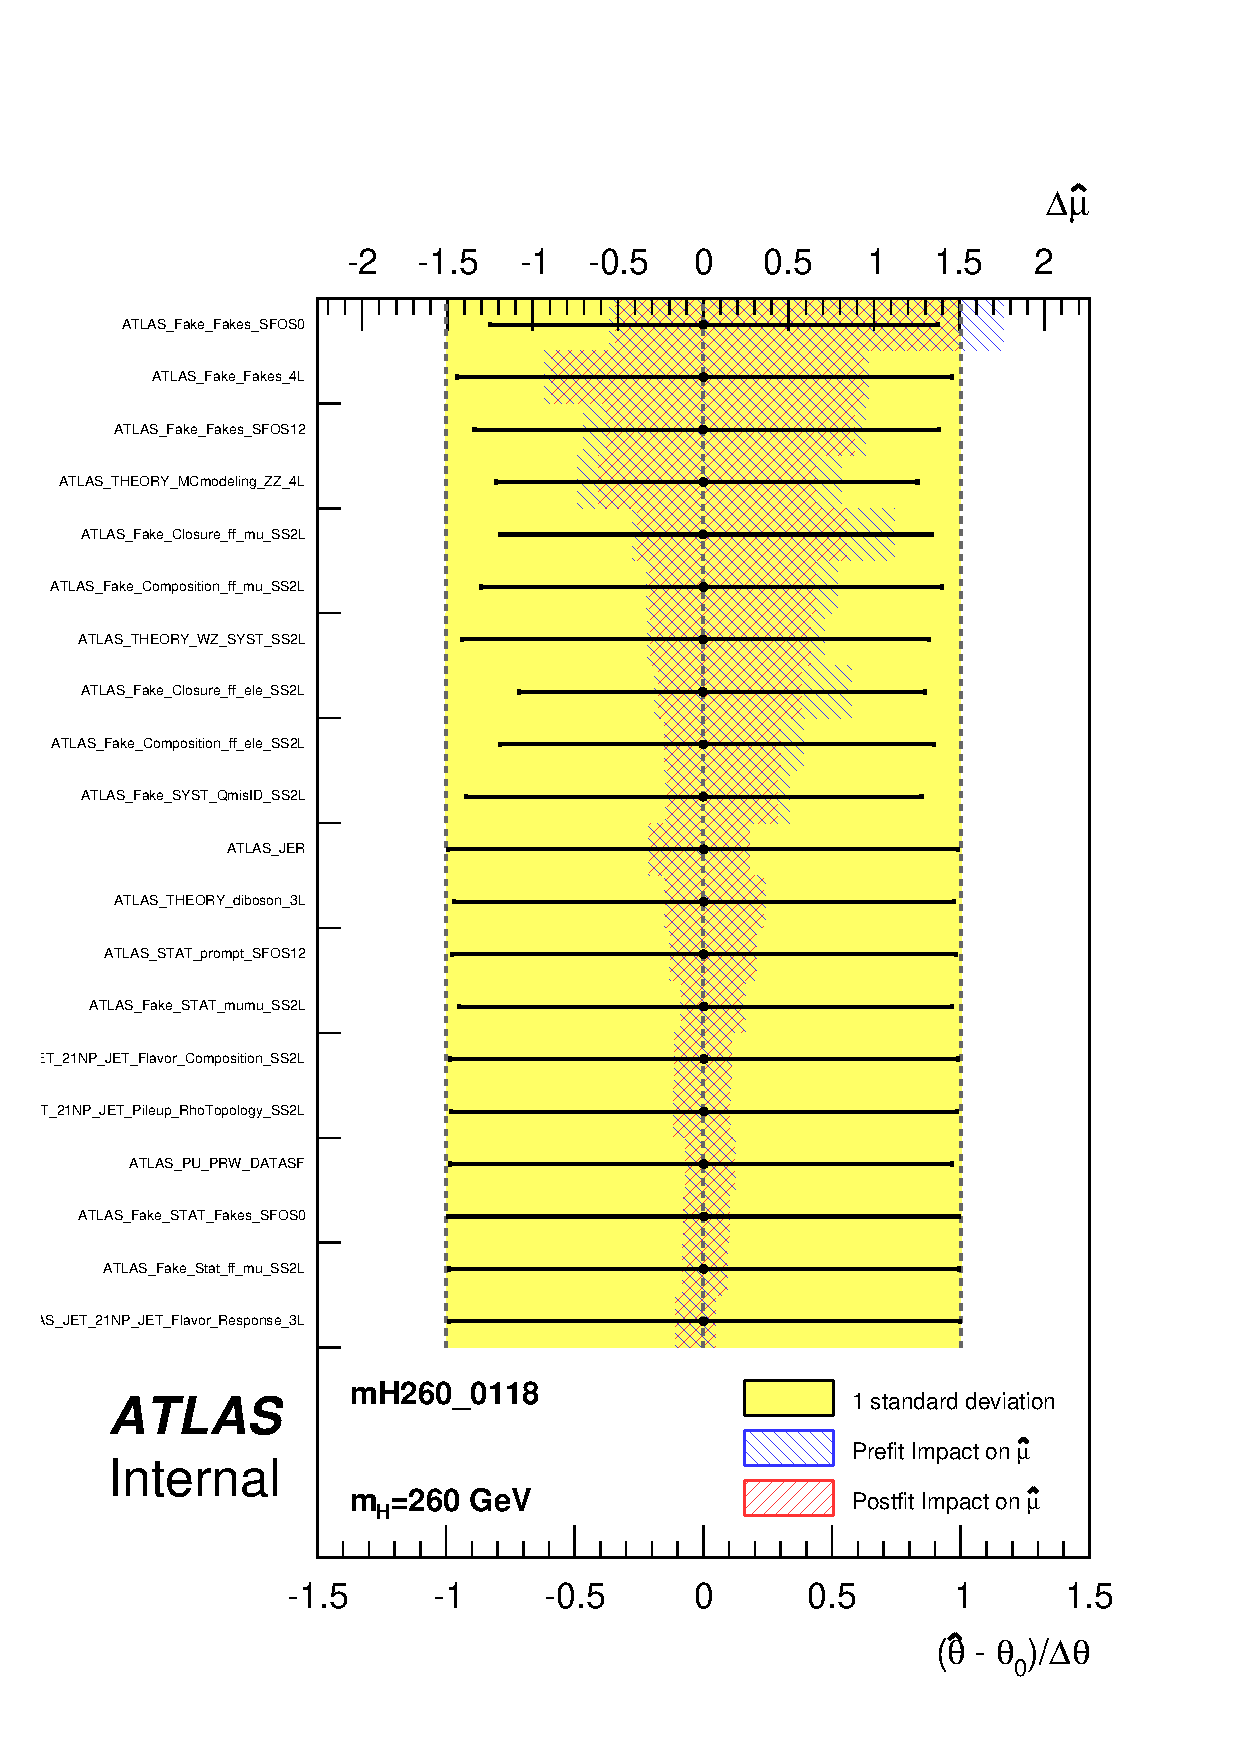
\includegraphics[width=.3\textwidth]{fig/Statistical/combination/rank-exp-combined-mH260.pdf}
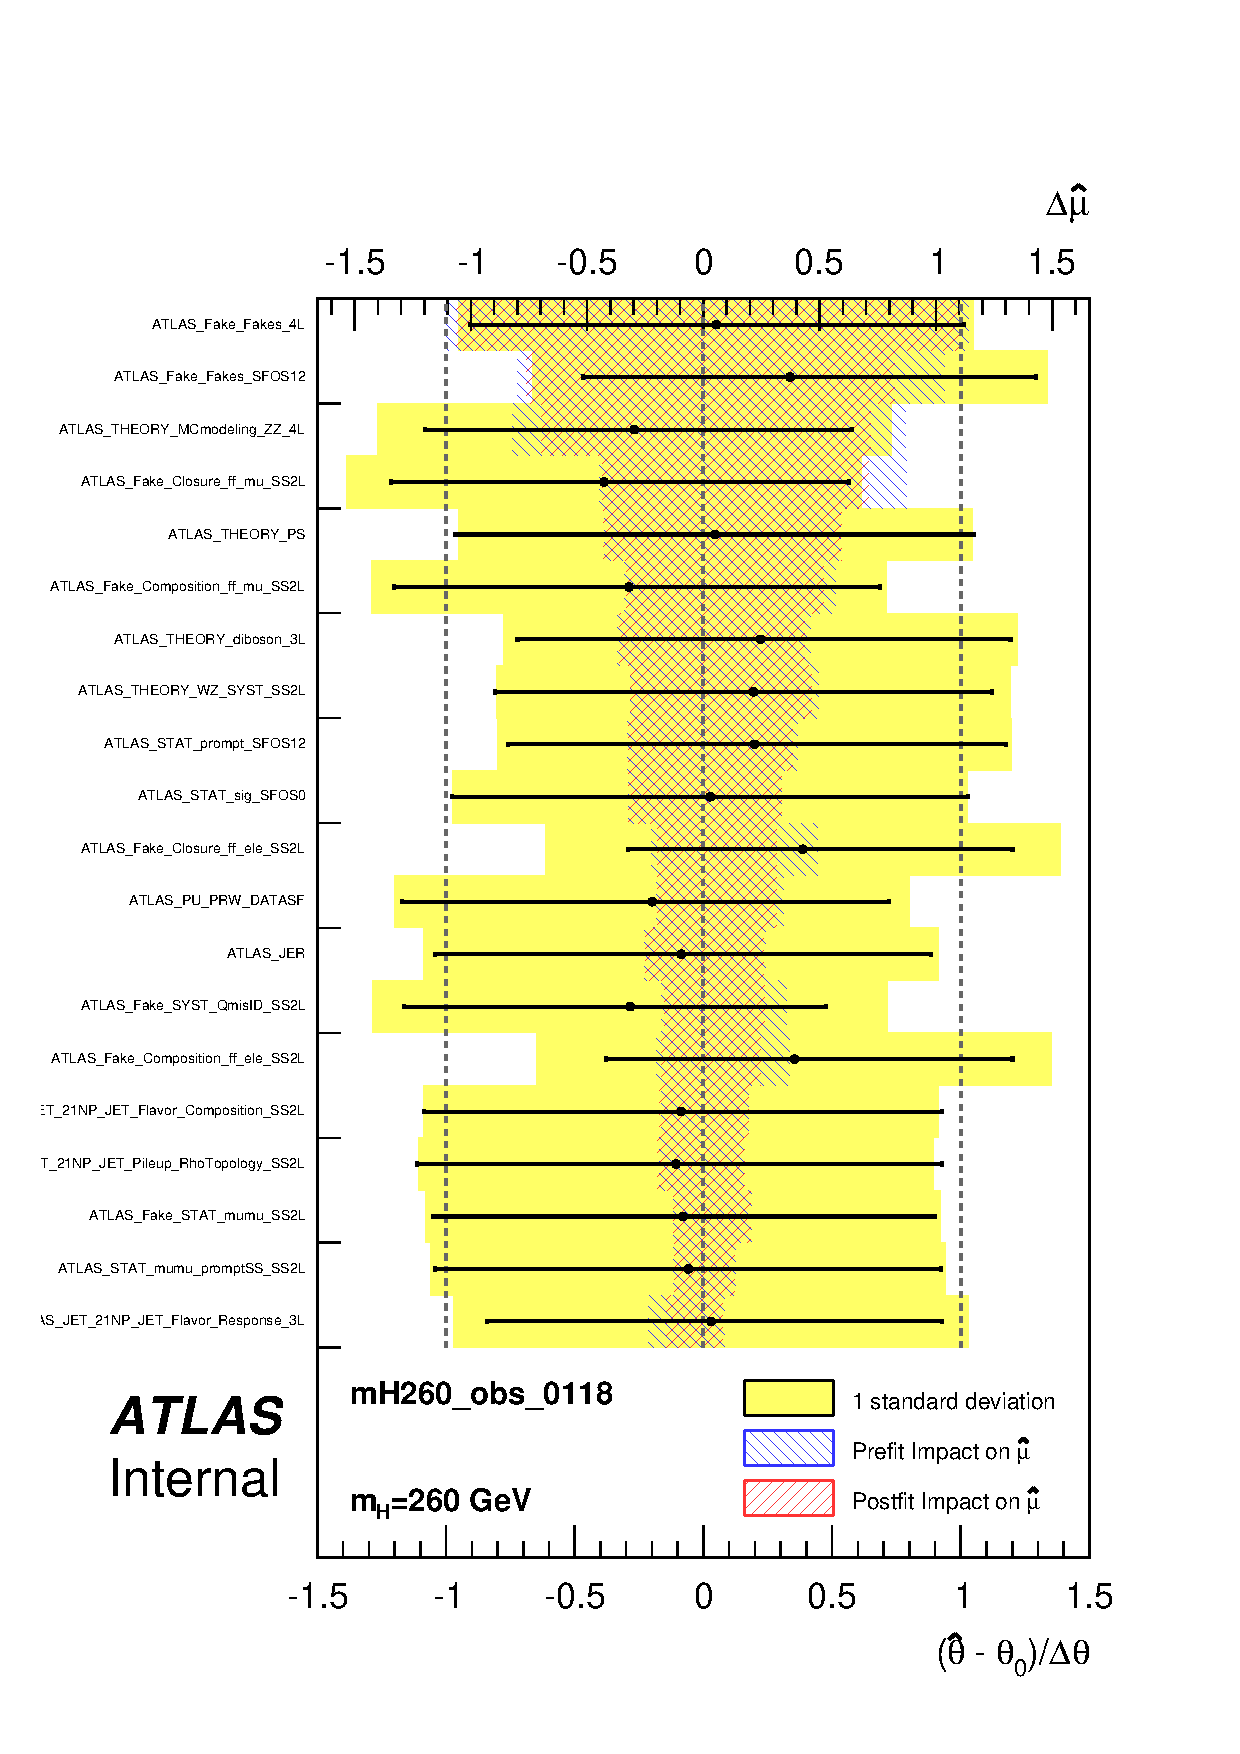
\includegraphics[width=.3\textwidth]{fig/Statistical/combination/rank-obs-combined-mH260.pdf}
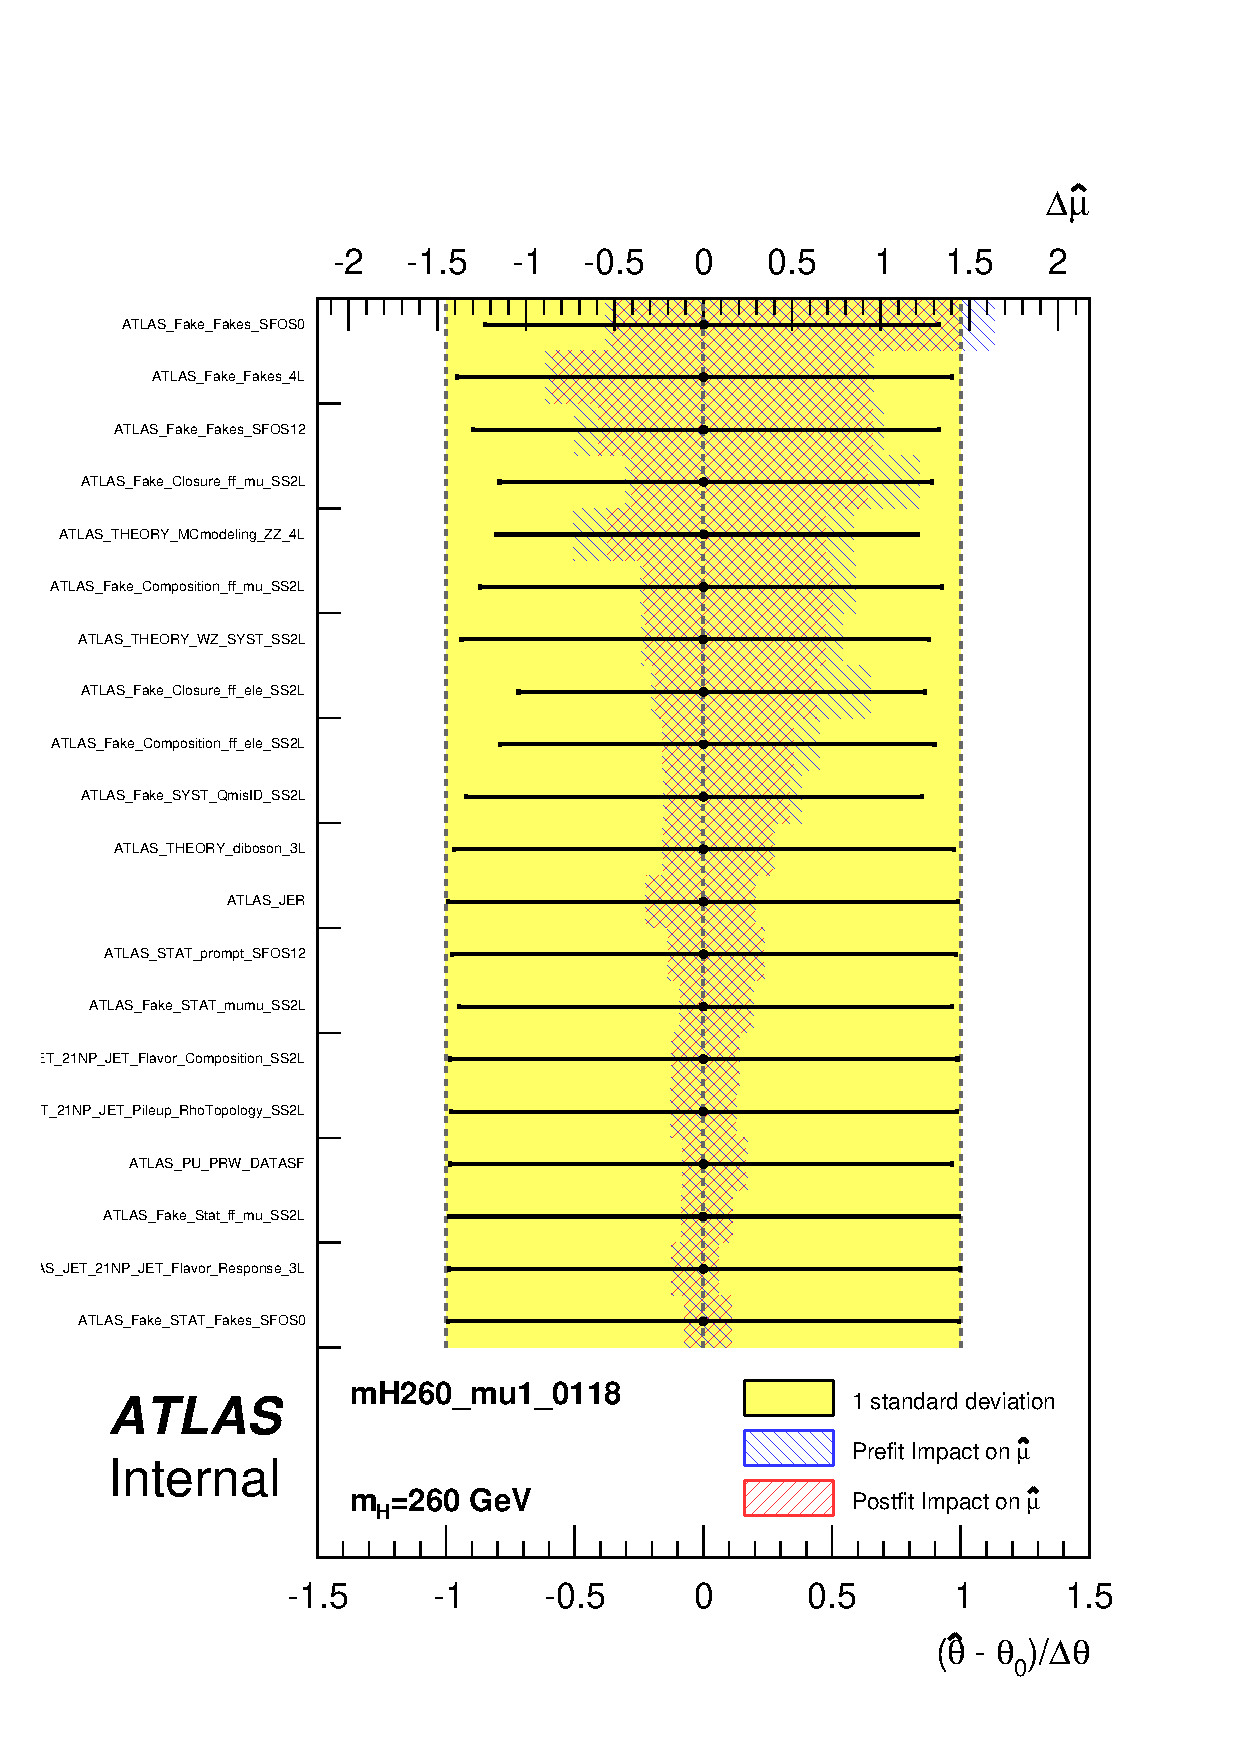
\includegraphics[width=.3\textwidth]{fig/Statistical/combination/rank-exp-combined-mH260_mu1.pdf}
%\caption{NP ranking check on B-only asimovData, obsData and S+B asimovData of $m_{H}=260 GeV$}
\caption{$m_X$=260 GeV分析NP影响排名,分别对应无信号Asimov数据,观测数据和S+B Asimov数据。}
\label{fig:rank-comb-260}
\end{figure}

\begin{figure}
\centering
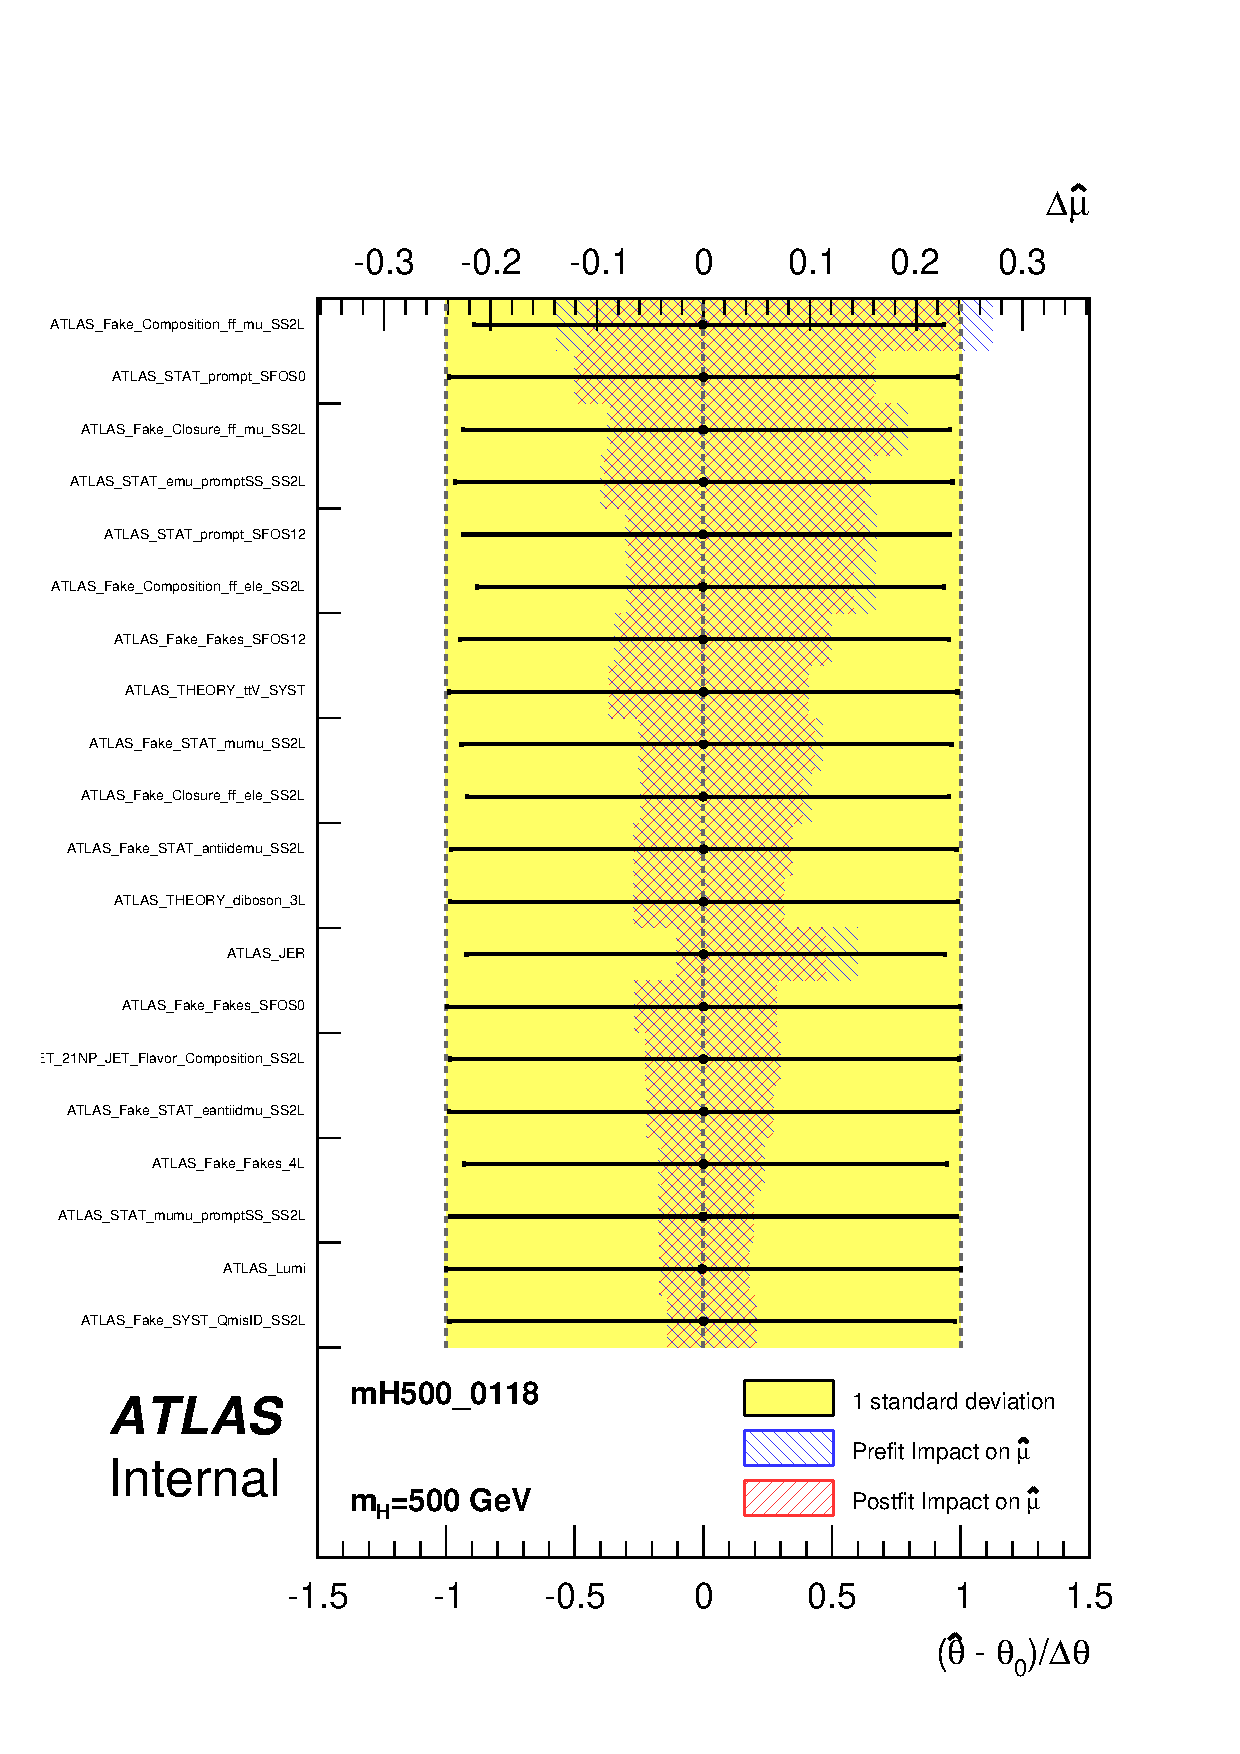
\includegraphics[width=.3\textwidth]{fig/Statistical/combination/rank-exp-combined-mH500.pdf}
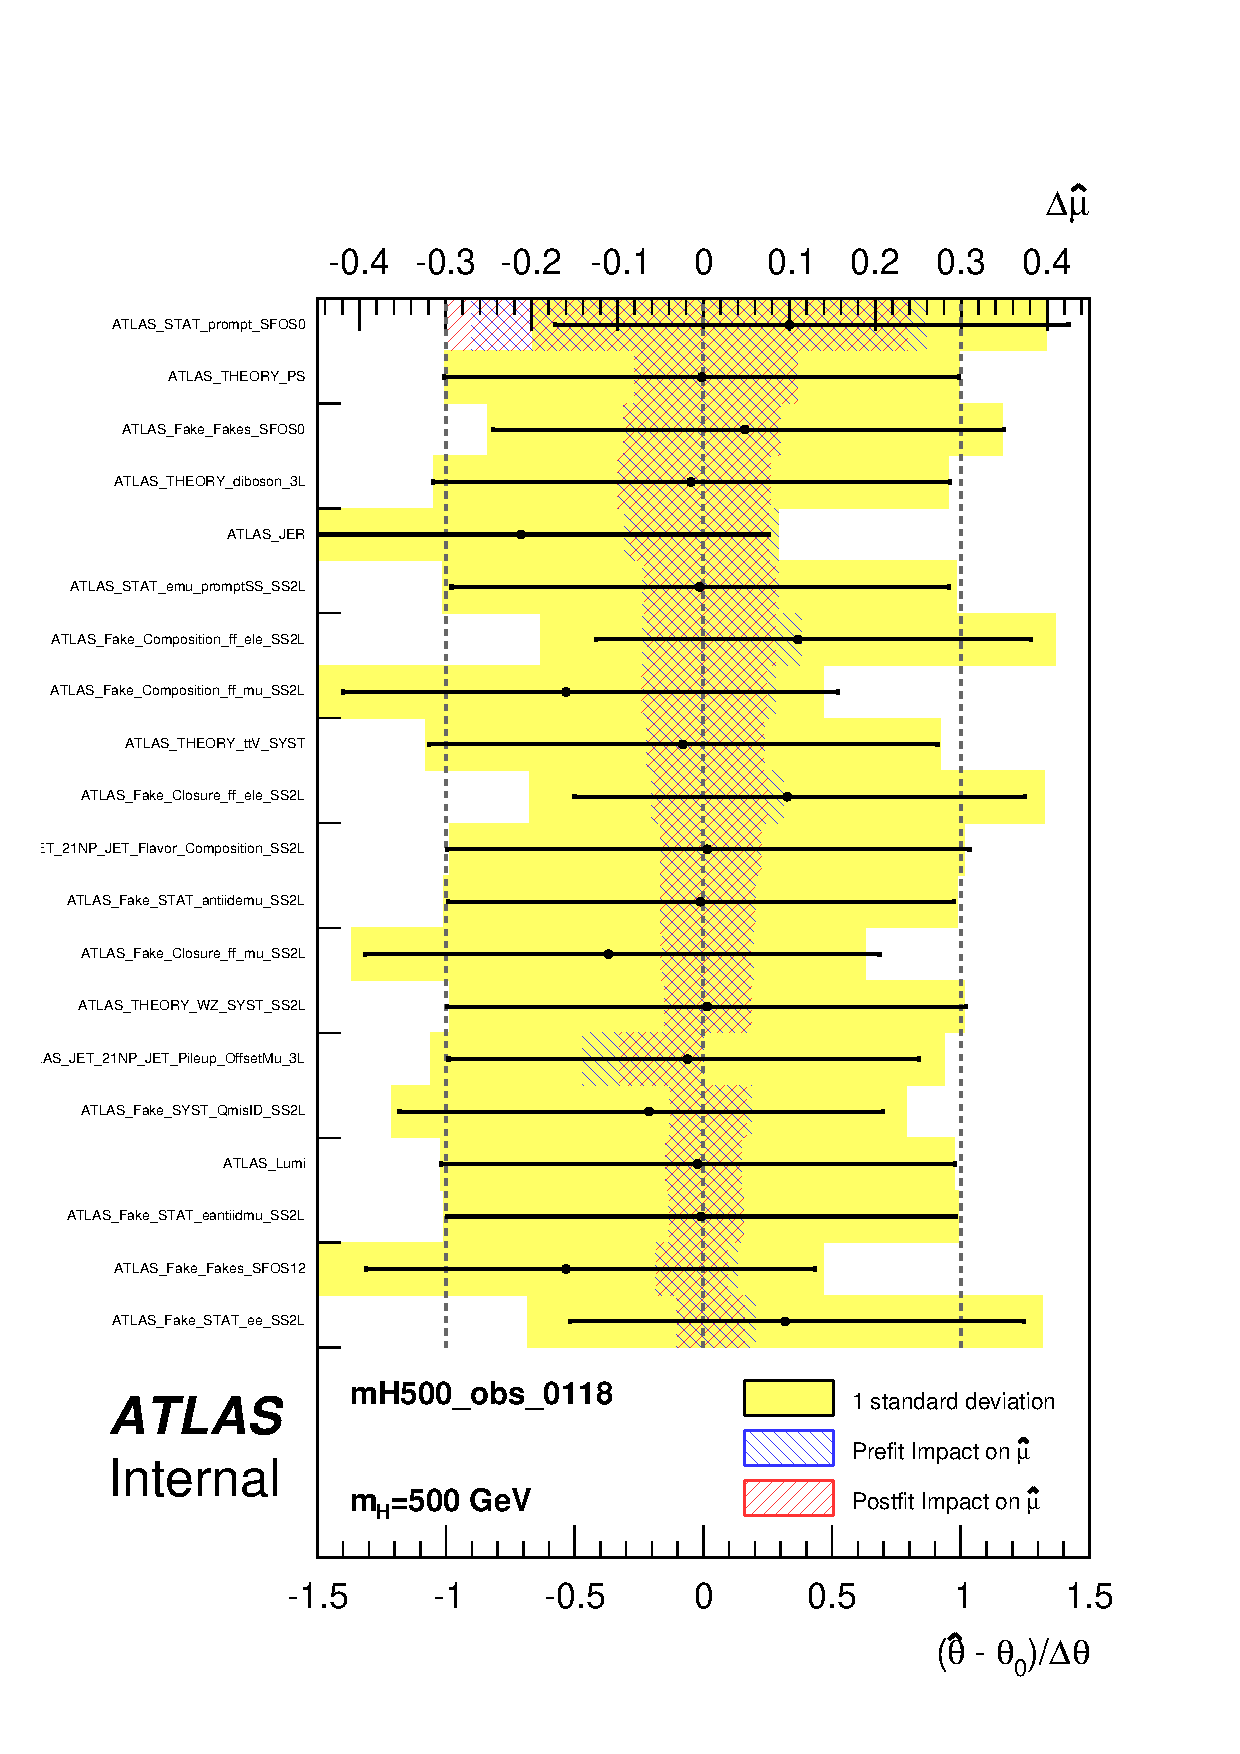
\includegraphics[width=.3\textwidth]{fig/Statistical/combination/rank-obs-combined-mH500.pdf}
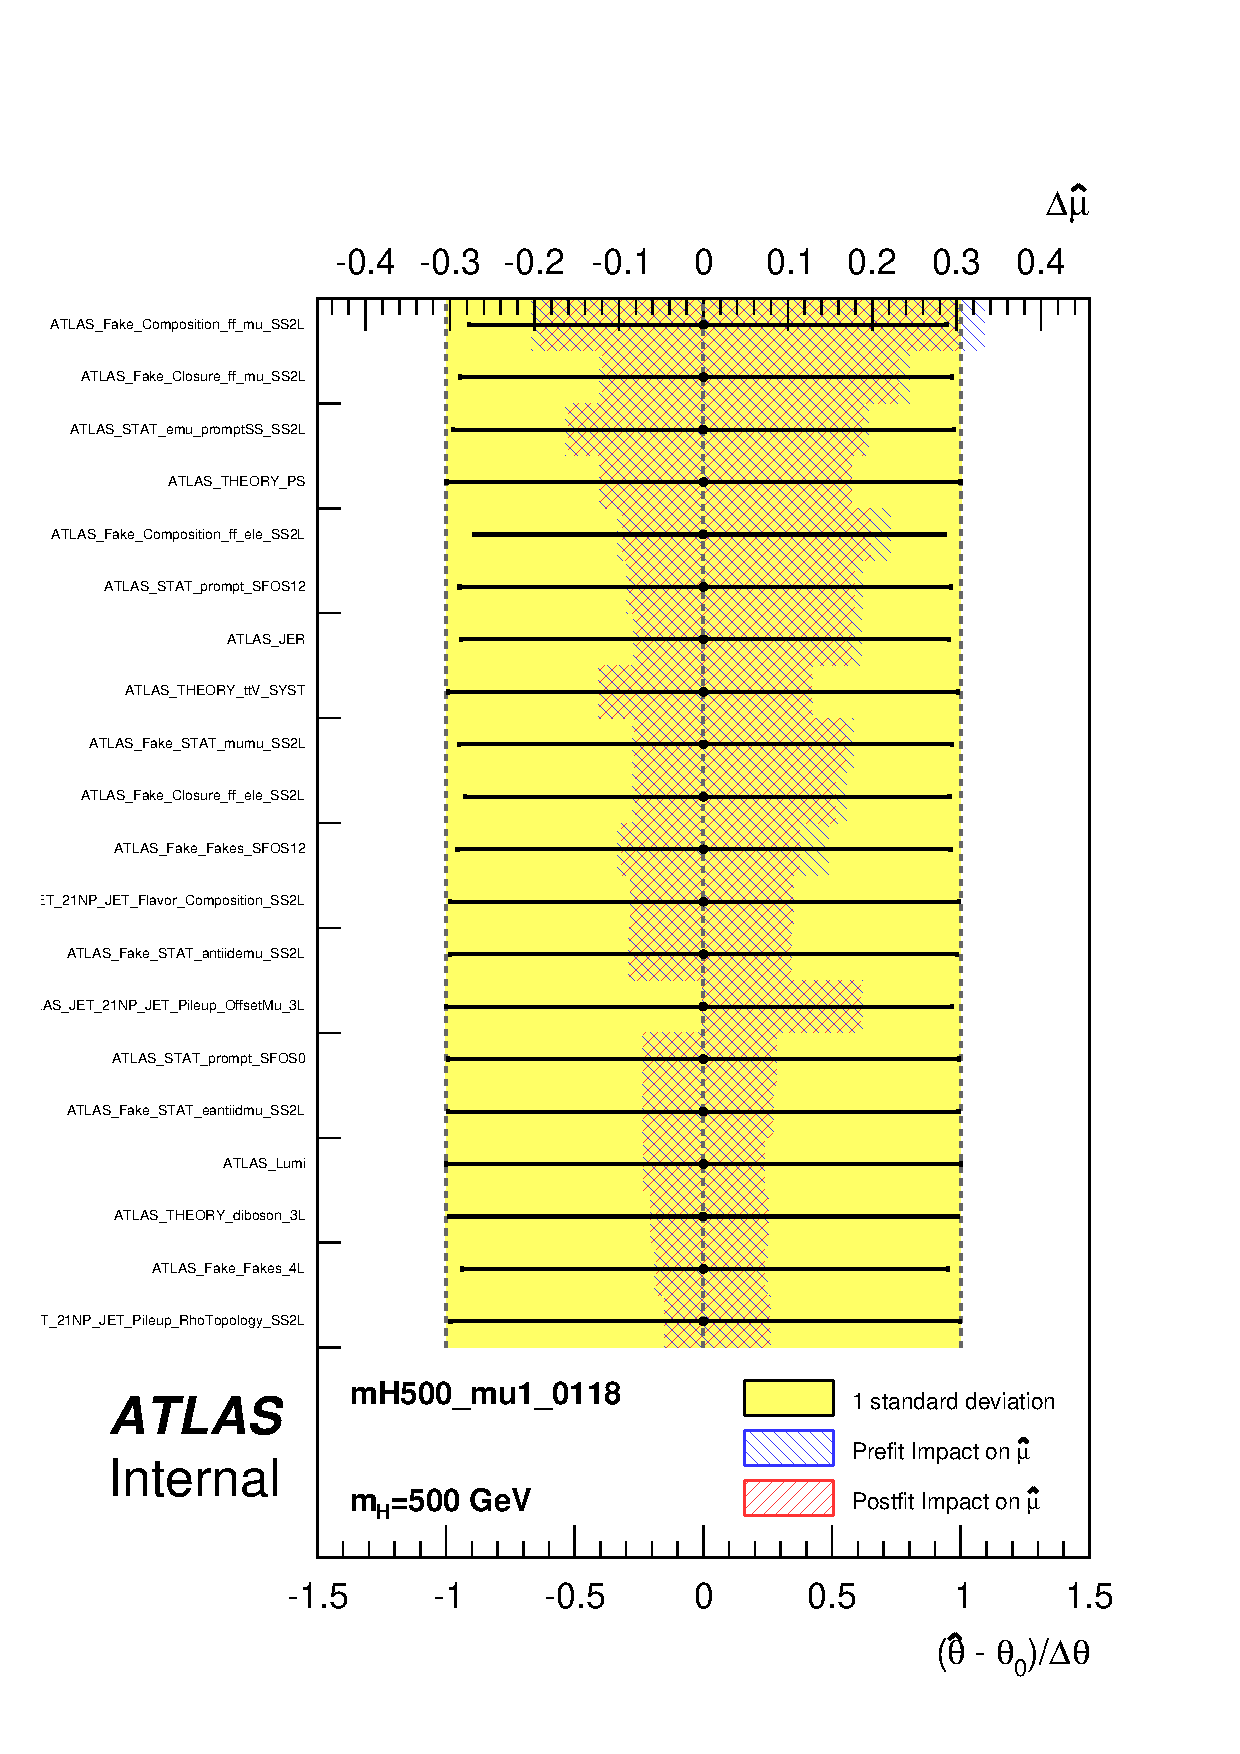
\includegraphics[width=.3\textwidth]{fig/Statistical/combination/rank-exp-combined-mH500_mu1.pdf}
%\caption{NP ranking check on B-only asimovData, obsData and S+B asimovData of $m_{H}=500 GeV$}
\caption{$m_X$=500 GeV分析NP影响排名,分别对应无信号Asimov数据,观测数据和S+B Asimov数据。}
\label{fig:rank-comb-500}
\end{figure}
%Another check is to fix specific uncertainty to nominal value and quantify the variation of upper limit compared with full systematics uncertainties. Table~\ref{tab:limit_withoutSys_hh}, \ref{tab:limit_withoutSys_SS_mH} and \ref{tab:limit_withoutSys_SS_mS} summarize the varition of upper limit after switching off certain uncertainty. The upper limit is sensitive to fake uncertainty.
%
\begin{table}
\centering
\begin{tabular}{|c|c|c|c|c|c|}
\hline
$\Delta limit/limit$	&nonres		&$m_{H}=260GeV$	&$m_{H}=300GeV$	&$m_{H}=400GeV$	&$m_{H}=500GeV$	\\
\hline
Lumi	&0.00	&0.01	&0.02	&0.03	&0.00\\
\hline
JET	&0.10	&0.02	&0.05	&0.11	&0.07\\
\hline
FT	&0.01	&0.01	&0.02	&0.03	&0.00\\
\hline
EG	&0.00	&0.01	&0.02	&0.03	&0.00\\
\hline
EL	&0.00	&0.01	&0.02	&0.03	&0.00\\
\hline
MUON	&0.00	&0.01	&0.02	&0.03	&0.00\\
\hline
MET	&0.00	&0.01	&0.02	&0.03	&0.00\\
\hline
MC STAT	&0.02	&0.01	&0.03	&0.04	&0.03\\
\hline
Fake	&0.08	&0.10	&0.12	&0.21	&0.11\\
\hline
THEORY	&0.05	&0.05	&0.06	&0.10	&0.04\\
\hline
\end{tabular}
\caption{$\Delta limit/limit$ is shown after switching off specific uncertainty in hh model}
\label{tab:limit_withoutSys_hh}
\end{table}


\begin{table}
\centering
\begin{tabular}{|c|c|c|c|c|c|}
\hline
$\Delta limit/limit$	&H280S135		&H300S145	&H320S155	&H340S135\\
\hline
Lumi	&0.004	&0.001	&0.006	&0.044\\
\hline
JET	&0.011	&0.031	&0.040	&0.086\\
\hline
FT	&0.003	&0.001	&0.004	&0.042\\
\hline
EG	&0.003	&0.001	&0.004	&0.041\\
\hline
EL	&0.003	&0.001	&0.004	&0.042\\
\hline
MUON	&0.003	&0.001	&0.004	&0.042\\
\hline
MET	&0.003	&0.000	&0.004	&0.042\\
\hline
MC STAT	&0.008	&0.007	&0.012	&0.051\\
\hline
Fake	&0.131	&0.154	&0.174	&0.190\\
\hline
THEORY	&0.030	&0.034	&0.045	&0.071\\
\hline
\end{tabular}
\caption{$\Delta limit/limit$ is shown after switching off specific uncertainty in SS model}
\label{tab:limit_withoutSys_SS_mH}
\end{table}



\begin{table}
\centering
\begin{tabular}{|c|c|c|c|c|c|}
\hline
$\Delta limit/limit$	&H340S135		&H340S145	&H340S155	&H340S165\\
\hline
Lumi	&0.044	&0.036	&0.029	&0.023\\
\hline
JET	&0.086	&0.075	&0.026	&0.006\\
\hline
FT	&0.042	&0.037	&0.031	&0.012\\
\hline
EG	&0.041	&0.037	&0.034	&0.000\\
\hline
EL	&0.042	&0.037	&0.034	&0.006\\
\hline
MUON	&0.042	&0.037	&0.034	&0.006\\
\hline
MET	&0.042	&0.037	&0.034	&0.000\\
\hline
MC STAT	&0.051	&0.037	&0.037	&0.006\\
\hline
Fake	&0.190	&0.275	&0.289	&0.234\\
\hline
THEORY	&0.071	&0.067	&0.055	&0.023\\
\hline
\end{tabular}
\caption{$\Delta limit/limit$ is shown after switching off specific uncertainty in SS model}
\label{tab:limit_withoutSys_SS_mS}
\end{table}


另一个重要检查是在拟合中固定住单个或者多个系统误差,观察结果变化。表~\ref{tab:limit_withoutSys_hh},表~\ref{tab:limit_withoutSys_SS_mH}和表~\ref{tab:limit_withoutSys_SS_mS}总结
在固定住某些系统误差后,拟合截面上限的变化,得出结论拟合结果对fakes的误差最敏感,与前述的影响排序是一致的。

\begin{table}
\centering
\begin{tabular}{|c|c|c|c|c|c|}
\hline
$\Delta limit/limit$	&nonres		&$m_{H}=260GeV$	&$m_{H}=300GeV$	&$m_{H}=400GeV$	&$m_{H}=500GeV$	\\
\hline
Lumi	&0.00	&0.01	&0.02	&0.03	&0.00\\
\hline
JET	&0.10	&0.02	&0.05	&0.11	&0.07\\
\hline
FT	&0.01	&0.01	&0.02	&0.03	&0.00\\
\hline
EG	&0.00	&0.01	&0.02	&0.03	&0.00\\
\hline
EL	&0.00	&0.01	&0.02	&0.03	&0.00\\
\hline
MUON	&0.00	&0.01	&0.02	&0.03	&0.00\\
\hline
MET	&0.00	&0.01	&0.02	&0.03	&0.00\\
\hline
MC STAT	&0.02	&0.01	&0.03	&0.04	&0.03\\
\hline
Fake	&0.08	&0.10	&0.12	&0.21	&0.11\\
\hline
THEORY	&0.05	&0.05	&0.06	&0.10	&0.04\\
\hline
\end{tabular}
\caption{$\Delta limit/limit$ is shown after switching off specific uncertainty in hh model}
\label{tab:limit_withoutSys_hh}
\end{table}


\begin{table}
\centering
\begin{tabular}{|c|c|c|c|c|c|}
\hline
$\Delta limit/limit$	&H280S135		&H300S145	&H320S155	&H340S135\\
\hline
Lumi	&0.004	&0.001	&0.006	&0.044\\
\hline
JET	&0.011	&0.031	&0.040	&0.086\\
\hline
FT	&0.003	&0.001	&0.004	&0.042\\
\hline
EG	&0.003	&0.001	&0.004	&0.041\\
\hline
EL	&0.003	&0.001	&0.004	&0.042\\
\hline
MUON	&0.003	&0.001	&0.004	&0.042\\
\hline
MET	&0.003	&0.000	&0.004	&0.042\\
\hline
MC STAT	&0.008	&0.007	&0.012	&0.051\\
\hline
Fake	&0.131	&0.154	&0.174	&0.190\\
\hline
THEORY	&0.030	&0.034	&0.045	&0.071\\
\hline
\end{tabular}
\caption{$\Delta limit/limit$ is shown after switching off specific uncertainty in SS model}
\label{tab:limit_withoutSys_SS_mH}
\end{table}



\begin{table}
\centering
\begin{tabular}{|c|c|c|c|c|c|}
\hline
$\Delta limit/limit$	&H340S135		&H340S145	&H340S155	&H340S165\\
\hline
Lumi	&0.044	&0.036	&0.029	&0.023\\
\hline
JET	&0.086	&0.075	&0.026	&0.006\\
\hline
FT	&0.042	&0.037	&0.031	&0.012\\
\hline
EG	&0.041	&0.037	&0.034	&0.000\\
\hline
EL	&0.042	&0.037	&0.034	&0.006\\
\hline
MUON	&0.042	&0.037	&0.034	&0.006\\
\hline
MET	&0.042	&0.037	&0.034	&0.000\\
\hline
MC STAT	&0.051	&0.037	&0.037	&0.006\\
\hline
Fake	&0.190	&0.275	&0.289	&0.234\\
\hline
THEORY	&0.071	&0.067	&0.055	&0.023\\
\hline
\end{tabular}
\caption{$\Delta limit/limit$ is shown after switching off specific uncertainty in SS model}
\label{tab:limit_withoutSys_SS_mS}
\end{table}

\clearpage

\subsection{联合统计结果}
最终提取出的$hh$95\% CL$_s$的截面上限如表~\ref{tab:limit-comb}和图~\ref{fig:limit-comb}所示。标准模型希格斯对
的观测(期望)截面上限值($pp\rightarrow hh$)为160倍(120倍)标准模型预测值;
共振态($pp\rightarrow X\rightarrow hh$)的观测(期望)截面上限值随着$m_X$增加从9.3 pb(10 pb)到2.8 pb(2.6 pb);
观测值均在一倍$\sigma$以内。
在低质量区,4L具有最高的期望显著性,3L次之,2LSS最低,而在高质量区,其顺序刚好相反。
在$SS$信号($pp\rightarrow SS$)搜寻中,所有质量点的观测值均在期望值的一个标准偏差以内,
观测(期望)截面上限值随$m_X$或$m_S$增大从
2.5 pb (2.5 pb)减小到0.16 pb(0.17 pb),
其中在低质量区4L同样地具有最高的显著性,而在高质量区三个分析道显著性非常接近。
\begin{figure}[!h!tpb]
  \centering
 %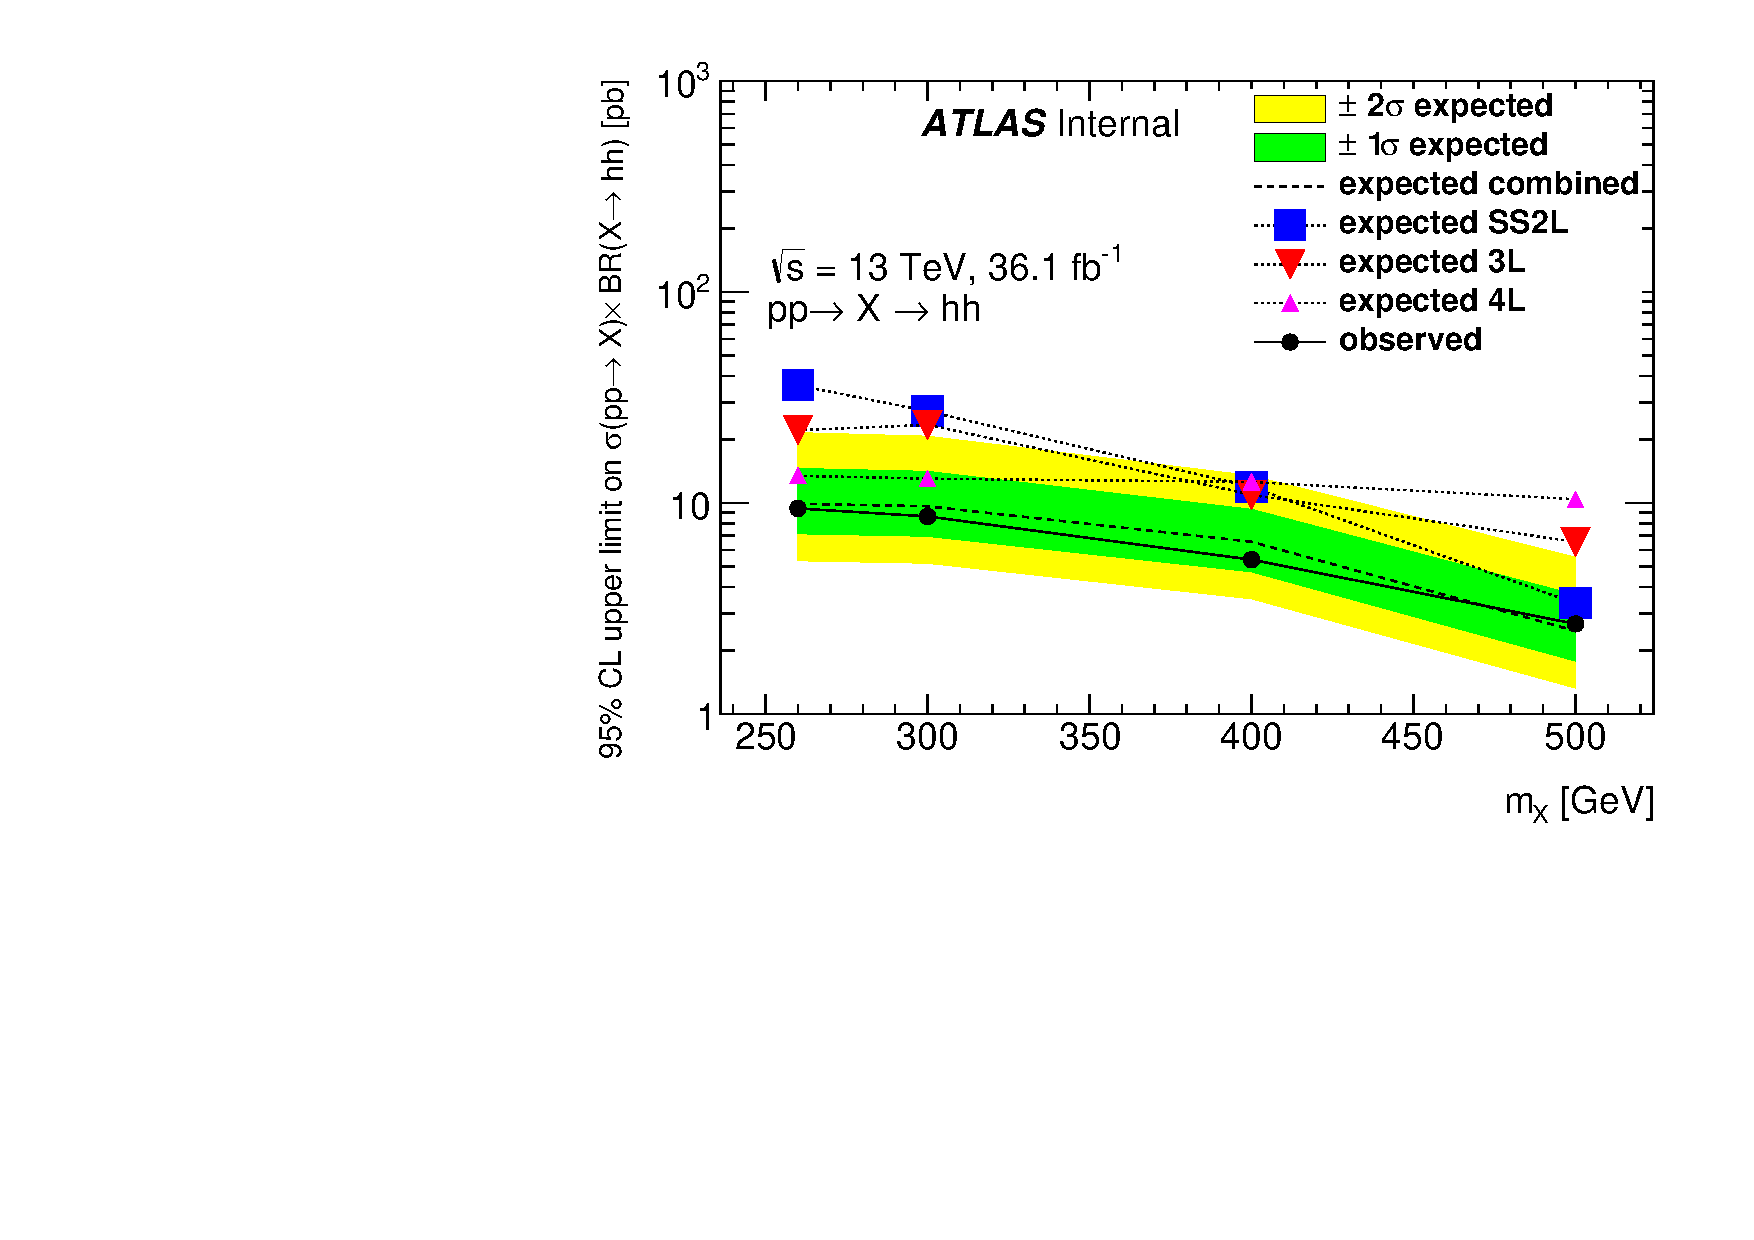
\includegraphics[width=0.65\textwidth,angle=-90]{fig/Statistical/combination/limit-comb-hh-AllSys.pdf}
 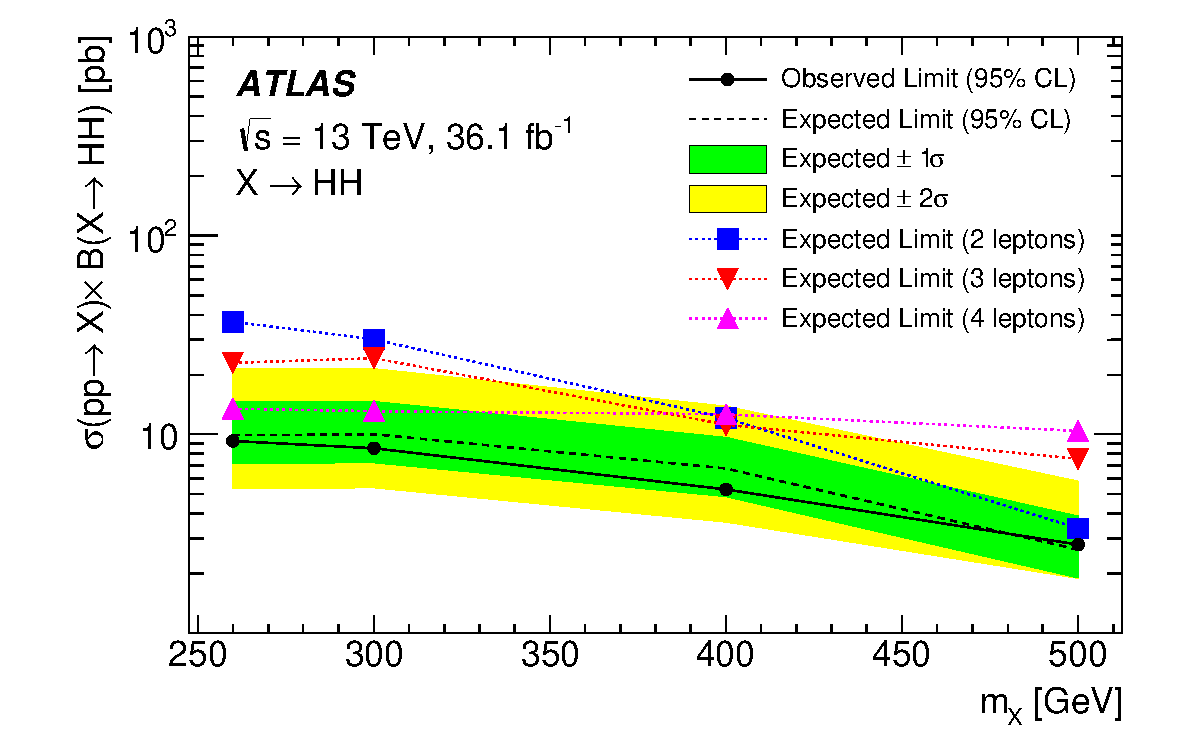
\includegraphics[width=0.75\textwidth]{fig/4W-Paper-36ifb_Paper_figures_limits_limit-comb-hh-AllSys.pdf}
 %\caption{The 95\% CL upper limits in $WWWW$ channels with all systematic.}
\caption{通过4W分析给出的$X\rightarrow hh$截面上限值(pb)随$m_X$分布,包括各个衰变道的期望值和联合结果。}
 \label{fig:limit-comb}
\end{figure}
\begin{table}[h]
\scriptsize
  \centering
%  \begin{tabular}{c|c|c|c|c|c}
%  \hline
%Upper Limit(pb) &non-resonant   &$m_{X}$ = 260 GeV        &$m_{X}$ = 300 GeV        &$m_{X}$ = 400 GeV        &$m_{X}$ = 500 GeV\\
%\hline
%expected 2L  &144.57 &27.60  &23.88  &9.77   &3.21   \\
%\hline
%expected 3L     &211.94 &20.38  &20.61  &10.26  &6.17   \\
%\hline
%expected 4L     &387.41 &13.44  &13.03  &12.56  &10.37  \\
%\hline
%combined        &111.42 &9.66   &9.41   &6.14   &2.41   \\
%\hline
%observed        &159.29 &9.09   &8.23   &5.19   &2.56   \\
%\hline
%+2$\sigma$     &215.30  &19.84  &19.11  &11.34  &5.08   \\
%\hline
%+1$\sigma$     &156.16  &13.90  &13.48  &8.40   &3.51   \\
%\hline
%-1$\sigma$     &80.28   &6.96   &6.78   &4.43   &1.74   \\
%\hline
%-2$\sigma$     &59.80   &5.18   &5.05   &3.30   &1.30   \\
%\hline
%\hline
%  \end{tabular}
%  \caption{This table summarizes the expected in each channel and combined channel and the combined observed limit. For non-resonant, the limit is on the ratio over SM Higgs pair prediction.}
\begin{tabular}{c c c c c c} 
    \hline
    & \multicolumn{1}{c}{\multirow{2}{*}{$\sigma/\sigma_{\text{SM}}$}} & \multicolumn{1}{c}{$m_X = 260$~GeV} & \multicolumn{1}{c}{$m_X = 300$~GeV} & \multicolumn{1}{c}{$m_X = 400$~GeV} & \multicolumn{1}{c}{$m_X = 500$~GeV} \\
    & & [pb] &  [pb] &  [pb] &  [pb]  \\
    \hline
    \hline
    Expected: 2 leptons &150 & 37 & 30 & 12 & 3.4 \\
    \hline
    Expected: 3 leptons & 270 & 23 & 24 & 11 & 7.5 \\
    \hline
    Expected: 4 leptons & 400 & 13 & 13 & 13 & 10 \\
    \hline
    \hline
    Expected & 120 & 9.9 & 10 & 6.7 & 2.6 \\
    \hline
    +2$\sigma$ & 230 & 21 & 21 & 14 & 5.8 \\
    \hline
    +1$\sigma$ & 170 & 15 & 15 & 9.7 & 3.9 \\
    \hline
    -1$\sigma$ & 83 & 7.1 & 7.2 & 4.9 & 1.9 \\
    \hline
    -2$\sigma$ & 62 & 5.3 & 5.4 & 3.6 & 1.4 \\
    \hline
    \hline
    Observed & 160 & 9.3 & 8.5 & 5.3 & 2.8 \\
    \hline
  \end{tabular}
\caption{通过4W分析给出的$X\rightarrow hh$截面上限值,包括各个衰变道的期望值和联合结果。}
%non-resonant的结果对应$\sigma/\sigma_{\text{SM}}$},其余对应截面(pb)。
  \label{tab:limit-comb}
\end{table}
\begin{figure}
  \centering
 \begin{subfigure}[b]{0.45\textwidth}
  %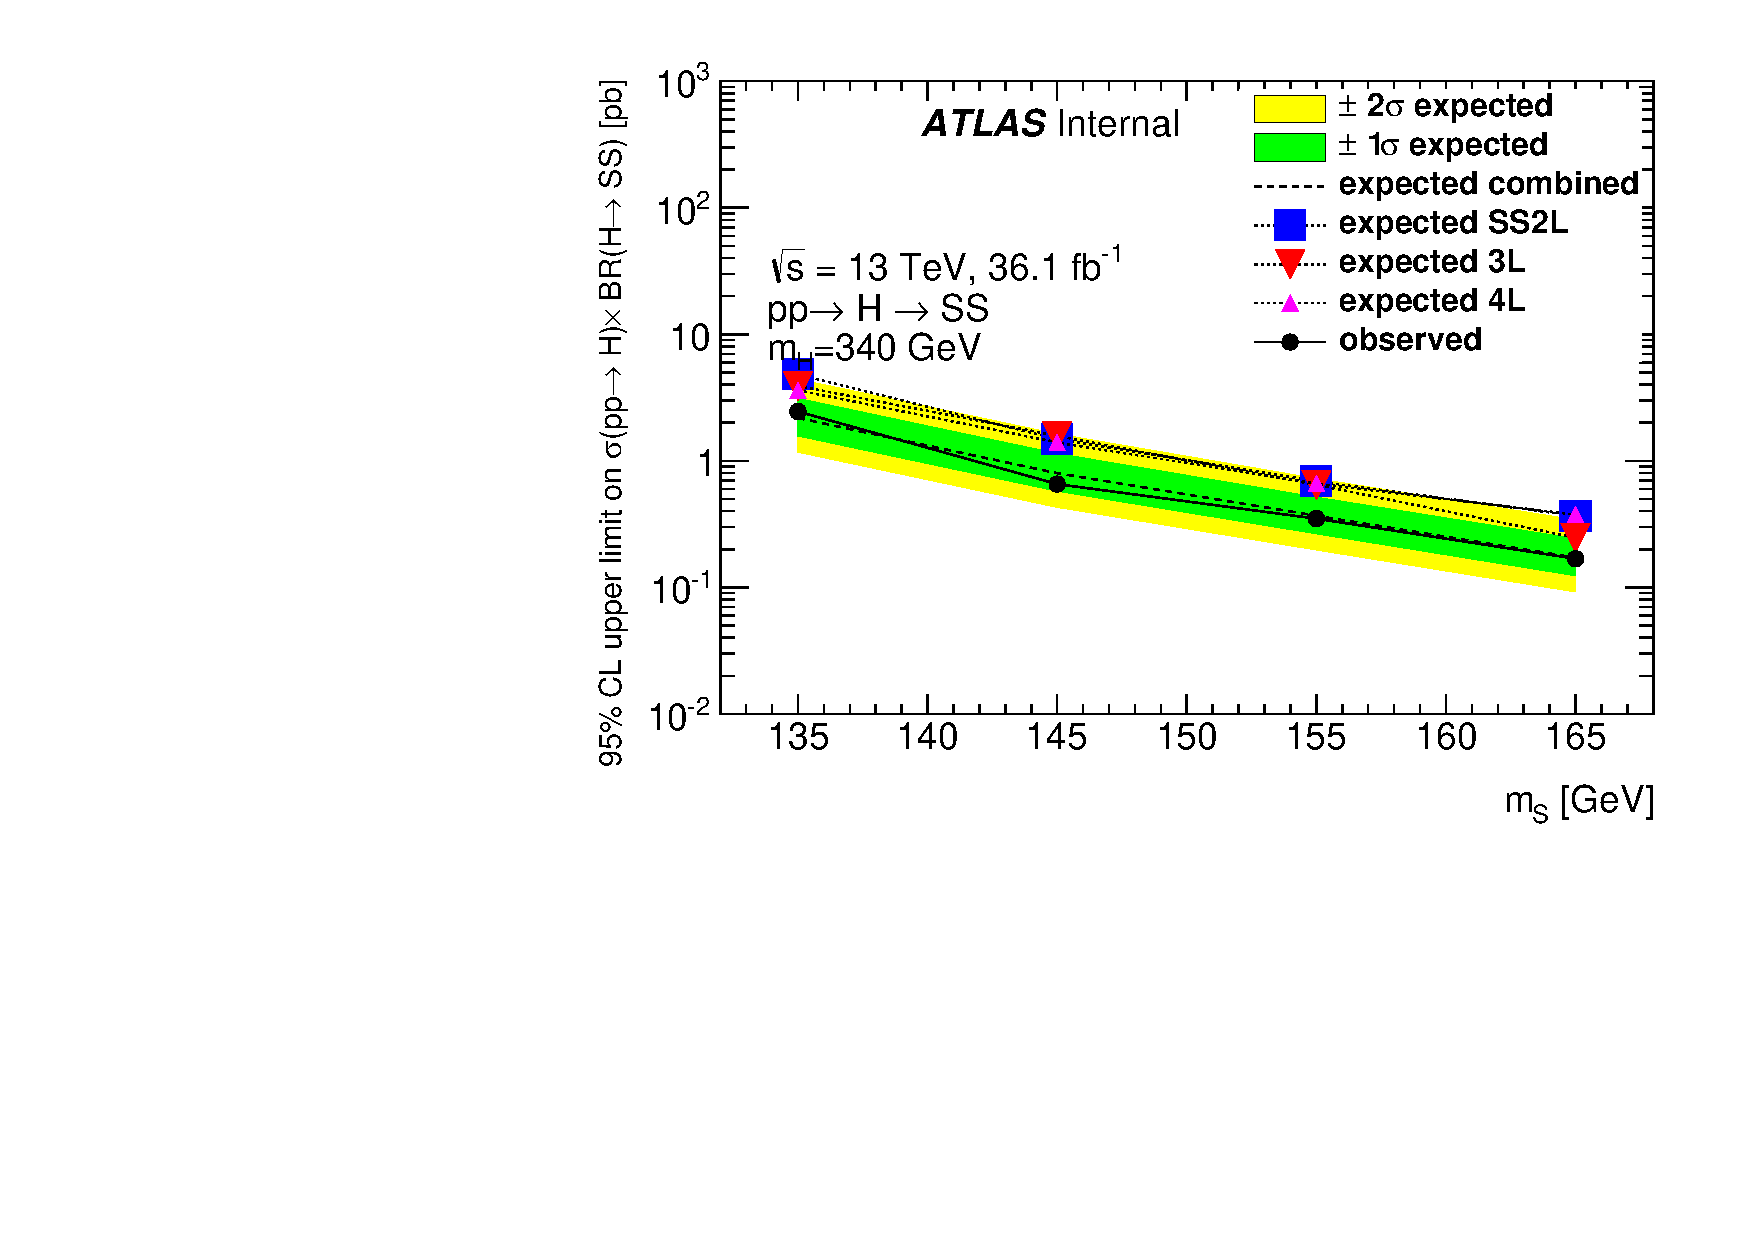
\includegraphics[width=.65\textwidth,angle=-90]{fig/Statistical/combination/limit-comb-SS-AllSys-mS.pdf}
  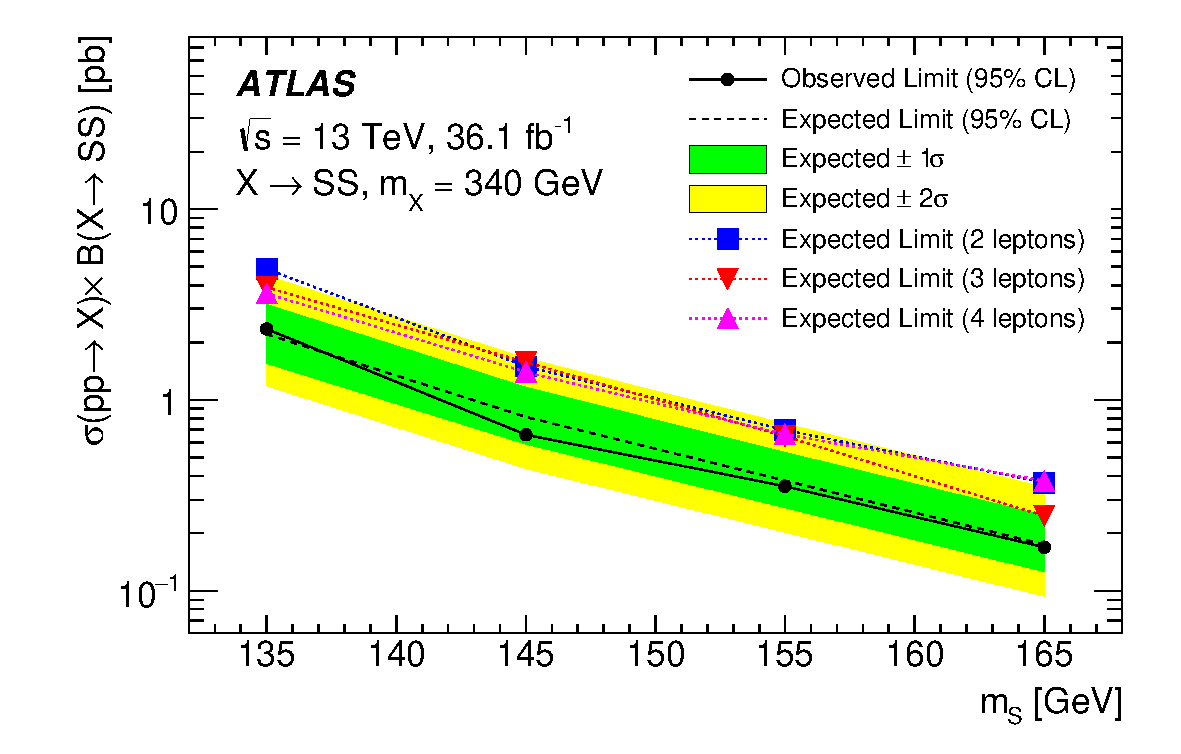
\includegraphics[width=.85\textwidth]{fig/4W-Paper-36ifb_Paper_figures_limits_limit-comb-SS-AllSys-mS.pdf}
 \end{subfigure}
 \begin{subfigure}[b]{0.45\textwidth}
  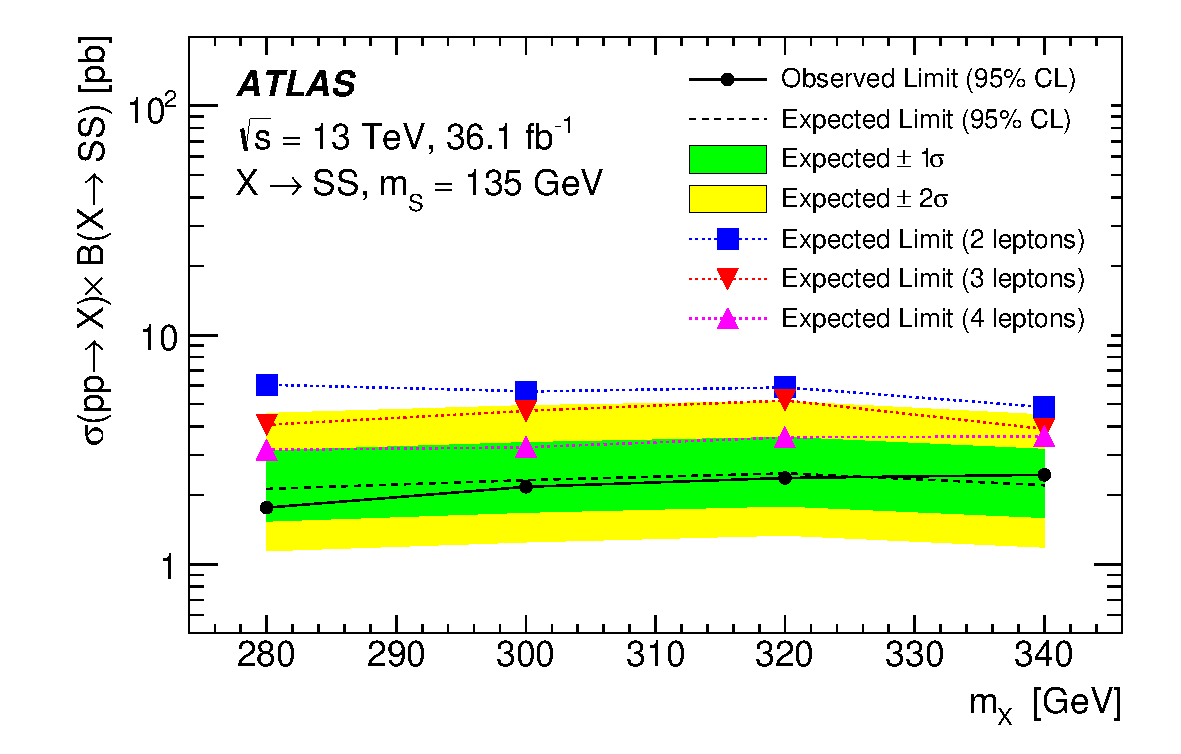
\includegraphics[width=.85\textwidth]{fig/4W-Paper-36ifb_Paper_figures_limits_limit-comb-SS-AllSys-mX.pdf}
 \end{subfigure}
  %\caption{The expected and observed limit with all systematic uncertainty is shown as the function of $m_{S}$}
  \caption{通过4W分析给出的$X\rightarrow SS$截面上限值(pb)随(a)~$m_S$与(b)~$m_X$分布,
包括各个衰变道的期望值和联合结果。}
  \label{fig:limit-comb-SS-mS}
\end{figure}
\begin{table}
\scriptsize
  \centering
%  \begin{tabular}{c|c|c|c|c|c|c|c}
%  \hline
%                &X280\_S135     &X300\_S135     &X320\_S135     &X340\_S135 &X340\_S145 &X340\_S155  &X340\_S165\\
%\hline
%expected SS 2L  &5.69   &5.41   &5.69   &4.83   &1.48   &0.69   &0.37   \\
%\hline
%expected 3L     &4.05   &4.67   &5.20   &3.90   &1.57   &0.65   &0.25   \\
%\hline
%expected 4L     &3.16   &3.25   &3.57   &3.61   &1.40   &0.66   &0.37   \\
%\hline
%combined        &2.20   &2.43   &2.53   &2.17   &0.92   &0.39   &0.19   \\
%\hline
%observed        &1.74   &2.15   &2.34   &2.45   &0.65   &0.35   &0.17   \\
%\hline
%+2$\sigma$     &4.46    &4.79   &5.13   &4.42   &1.63   &0.72   &0.34   \\
%\hline
%+1$\sigma$     &3.07    &3.33   &3.58   &3.12   &1.14   &0.52   &0.24   \\
%\hline
%-1$\sigma$     &1.52    &1.66   &1.80   &1.57   &0.58   &0.26   &0.12   \\
%\hline
%-2$\sigma$     &1.13    &1.24   &1.34   &1.17   &0.43   &0.20   &0.09   \\
%\hline
%  \end{tabular}
  \begin{tabular}{ccccc}
    \hline
    & $m_X = 280$~GeV & $m_X = 300$~GeV & $m_X = 320$~GeV & $m_X = 340$~GeV \\
         & [pb] &  [pb] &  [pb] &  [pb]  \\
    \hline
    \hline
    Expected: 2 leptons & 6.1 & 5.7 & 5.9 & 4.9 \\
    \hline
    Expected: 3 leptons & 4.1 & 4.7 & 5.2 & 3.9 \\
    \hline
    Expected: 4 leptons & 3.2 & 3.2 & 3.6 & 3.6 \\
    \hline
    \hline
    Expected & 2.1 & 2.3 & 2.5 & 2.2 \\
    \hline
    +2$\sigma$ & 4.6 & 4.9 & 5.1 & 4.5 \\
    \hline
    +1$\sigma$ & 3.1 & 3.4 & 3.6 & 3.2 \\
    \hline
    -1$\sigma$ & 1.5 & 1.7 & 1.8 & 1.6 \\
    \hline
    -2$\sigma$ & 1.1 & 1.3 & 1.3 & 1.2 \\
    \hline
    \hline
    Observed & 1.8 & 2.2 & 2.4 & 2.5 \\
    \hline
  \end{tabular}
%  \caption{This table shows the expected limit in each channel and the observed limit in $pp\rightarrow SS$ model.}
 \caption{通过4W分析给出的$X\rightarrow SS$截面上限值,对应$m_S=135$ GeV,包括各个衰变道的期望值和联合结果。}
  \label{tab:limit-comb-SS-mS}
\end{table}
\begin{table}[h]
\scriptsize
  \centering
  \begin{tabular}{cccc} 
    \hline
    & \multicolumn{1}{c}{$m_{S} = 145$~GeV} & \multicolumn{1}{c}{$m_{S} = 155$~GeV} & \multicolumn{1}{c}{$m_{S} = 165$~GeV} \\
        &  [pb] &  [pb] &  [pb]  \\
    \hline
    \hline
    Expected: 2 leptons & 1.5 & 0.69 & 0.37 \\
    \hline
    Expected: 3 leptons & 1.6 & 0.65 & 0.25 \\
    \hline
    Expected: 4 leptons & 1.4 & 0.66 & 0.37 \\
    \hline
    \hline
    Expected & 0.82 & 0.38 & 0.17 \\
    \hline
    +2$\sigma$ & 1.7 & 0.75 & 0.35 \\
    \hline
    +1$\sigma$ & 1.2 & 0.53 & 0.25 \\
    \hline
    -1$\sigma$ & 0.59 & 0.27 & 0.13 \\
    \hline
    -2$\sigma$ & 0.44 & 0.20 & 0.094 \\
    \hline
    \hline
    Observed & 0.66 & 0.35 & 0.16 \\
    \hline
  \end{tabular}
 \caption{通过4W分析给出的$X\rightarrow SS$截面上限值,对应$m_X=340$ GeV,包括各个衰变道的期望值和联合结果。}
  \label{tab:limit-comb-SS-mX}
\end{table}

